\documentclass[oneside]{book}

\usepackage{Style/Diagrams}
\usepackage{Style/Master}
\usepackage{Style/boxes}
\usepackage{Style/DefNoteFact}
\usepackage{Style/QnsProof}
\usepackage{Style/Thms}
\usepackage{Style/Env}
\usepackage{Style/NewCommands}

\newcommand{\highlight}[2][red!50]{\mathpalette{\highlightwithstyle[#1]}{#2}}
\newcommand{\highlightwithstyle}[3][red!50]{
  \begingroup                         %% <- limit scope of \box0 and \fboxsep assignment
    \sbox0{$\mathsurround 0pt #2#3$}% %% <- typeset content in box 0
    \setlength{\fboxsep}{.5pt}        %% <- set (smaller) framebox margins
    \sbox2{\hspace{-.5pt}%            %% <- create box 2, undo margin
      \colorbox{#1}{\usebox0}%        %% <- print the contents of box 0 in a \colorbox
    }%
    \dp2=\dp0 \ht2=\ht0 \wd2=\wd0     %% <- set dimensions of box 2 to match box 0
    \box2                             %% <- print box 2
  \endgroup                           %% <- revert old definitions of the boxes and \fboxsep
}   

\begin{document}

\begin{titlepage}
    \frontmatter
    \begin{tikzpicture}[font=\sffamily,remember picture,overlay]
        \node[fill=Dandelion,anchor=north, minimum width=\paperwidth, minimum height=2cm] (names)
     at ([yshift=0]current page.north) {
      \begin{tabular}{c}
          \\
          \color{blue} {\fontsize{24.88pt}{65pt}\selectfont A-Levels Physics Notes}\\[2mm]
          \Large \color{blue}{By Grass}\\
          \color{blue} {\fontsize{10pt}{10pt}\selectfont Licensed under the GNU General Public License v3.0}\\
      \end{tabular}
      };
    \end{tikzpicture}

\begingroup
\let\clearpage\relax
\vspace{2cm}
\tableofcontents
\endgroup
\mainmatter
\end{titlepage}

\chapter{Inequalities and Equations}
\section{Solving Inequalities}
\begin{stbox}{General Methods}
  \begin{enumerate}
    \item Quadratic formula for factorisation / finding roots (of polynomial).
    \item Completing the square.
    \item Discriminant/Completing the square to eliminate factors which are \emph{always} positive or negative (e.g. removing \(x^2-3x+4\)). \emph{Note to include coefficient of \(x^2\) in the argument.}
    \item GC (include sketch).
    \item \emph{Rational Functions}: Move everything to one side by adding or subtracting, then use a number line.
\end{enumerate}
\end{stbox}
\section{Modulus Inequalities}
\begin{fact}
    Given \(x \in \mathbb{R}\), we have that 
    \begin{itemize}
        \item \(\lvert x \rvert \geq 0\),
        \item \(\lvert x^2 \rvert=\lvert x \rvert^2=x^2\),
        \item \(\sqrt{x^2}=\lvert x \rvert\).
    \end{itemize}
    And as long as \(x \in \mathbb{R}^+\),
    \begin{itemize}
        \item \(\sqrt{x}^2=\lvert x \rvert\).
    \end{itemize}
\end{fact}
\begin{stbox}{Useful Properties}
  For every \(x,k \in \mathbb{R}\):
  \begin{enumerate}[label=(\alph*)]
      \item \(\lvert x \rvert < k\) iff \(-k<x<k\).
      \item \(\lvert x \rvert > k\) iff \(x<-k\) or \(x>k\).
  \end{enumerate}
\end{stbox}

\section{System of Linear Equations}
\begin{stbox}{General Information}
  \begin{itemize}
    \item  For more complicated real-world-context qns, try playing around with the values (e.g. use simultaneous equations) first. It may work out nicer than expected.
  \end{itemize}
\end{stbox}
\section{Summary}

\begin{lbox}[colbacktitle=white, coltitle=black, colframe=black]{G.C. Skills} 
  \begin{enumerate}
    \item Plotting curves \(y=f(x)\) in G.C.
    \item How to use simultaneous equation solver.
  \end{enumerate}
\end{lbox}
\begin{IN}
  \begin{itemize}
    \item Eliminating Factors --- \emph{only} works for \(c=0\) in \(f(x) \geq c\) or \(f(x) \leq c\).

    Counterexample: It is false that \(P(x)=x(3x^2-9x+10) \leq 2\) iff \(x \leq 2\). Notice that \(P(1.8)=6.336 \not\leq 2\). 
    \item Discriminant --- include coefficient of \(x^2\) in argument.
    \item When using factor elimination to remove some \(f(x)\), we only need to say that ``\(f(x)\) is negative''.
    \item Rational functions --- exclude the values that causes division by zero to occur.
    \item With inequalities, be really careful about multiplication! If \(x>y\) \emph{and} \hly{\(z>0\)}, then \(xz>yz\). 
    \item Cross multiplication preserves order for \(\frac{x}{y}<\frac{x'}{y'}\) iff \(y\) and \(y'\) are \emph{both} positive or negative.
    
    Note the counterexample \(\frac{1}{2}<\frac{1}{-3}\).
    \item Squaring preserves/reverses order for \(x<y\) iff \(x\) and \(y\) are \emph{both} positive or negative.
    \item Can't necessarily use differentiation to solve if qns asks for algebraic method.
    \item Safer to graph out the two functions separately!
    \item Be careful about whether to include equality! Don't forget to account for it!
    \item  Note that when solving for \(\lvert x \rvert=y\), \(\lvert x \rvert < y\), etc, \(y\) must be greater than or equal to 0. In other words, there may be solutions we will need to reject.
    \item Carelessness: Look at the question carefully! If they ask for a \emph{set} of values, then rmb to give it as a \emph{set}!
    \item Exponentiation and Logarithms: Simply use \(\ln\) and avoid \(\log_c\) for \(c<1\).
    
    Order is \emph{Preserved} under exponentiation/logarithms if the base is \emph{larger than} one. Otherwise, when it is \emph{less than} one, the order is \emph{reversed}. \url{https://www.desmos.com/calculator/gd8z5fa0bg}
    \item  For more complicated real-world-context qns, try playing around with the values (e.g. use simultaneous equations) first. It may work out nicer than expected.
\end{itemize}
\end{IN}

\chapter{Sequences and Series}
\section{Binomial Theorem and Series}
\begin{theorem}{The Binomial Theorem}{}
  \[(a+b)^n=\sum_{r=0}^{n}{\binom{n}{r}a^{n-r}b^r},\]
  where \(n \in \mathbb{Z}^{+}\).
\end{theorem}
\begin{theorem}{The Binomial Series}{}
  \[(1+x)^{p}=\sum_{r=0}^{\infty}{\binom{p}{r}x^r},\]
  where \(p \in \mathbb{Q}\), \(\lvert x \rvert<1\), and
  \[\binom{p}{r}:=\frac{p(p-1)\cdots(p-r+1)}{r!}.\]
\end{theorem}
\begin{corollary}{}{}
  Clearly,
  \[(a+x)^p=a^p\left(1+\frac{x}{a}\right)^p=a^p \sum_{r=0}^{\infty}{\binom{p}{r}\frac{x^r}{a^r}},\]
  under the same conditions.
\end{corollary}
\begin{fact}
  We can expand \((a+x)^p\) in descending powers of \(x\) by using \((a+x)^p=x^p\left(1+\frac{a}{x}\right)^p\).
\end{fact}
\begin{note}
  Sometimes computing a couple terms can be useful in finding a pattern. For example, to get the coefficient of \(x^k\) explicitly.
\end{note}
\newpage
\section{APGP}
\begin{stbox}{Basics}{}
    \begin{center}
    \begin{tabular}{|Sc|Sc|Sc|}
    \hline
    & AP & GP\\
    \hline
    \multirow{2}{*}{\(u_n\)} & \multicolumn{2}{Sc|}{\(u_n=S_n-S_{n-1}\)}\\
    \cline{2-3}
    & \(u_n=a+(n-1)d\) & \(u_n=ar^{n-1}\)\\
    \hline
    \(S_n\) & 
    \begin{tabular}{@{}Sc@{}} 
      \(S_n=\frac{n}{2}[2a+(n-1)d]\)\\
      \(=\frac{n}{2}(a+\ell)\hspace{0.7cm}\)
    \end{tabular} & 
    \begin{tabular}{@{}Sc@{}}
      \(S_n=\frac{a\left(1-r^n\right)}{1-r}\)\\
      \(\hphantom{S_n}=\frac{a\left(r^n-1\right)}{r-1}\)
    \end{tabular}\\
    \hline
    \(S_\infty\) & Divergent & Converges to \(S_\infty=\frac{a}{1-r}\) \footnotesize when \(\lvert r \rvert<1\).\normalsize\\
    \hline
    Prove AP/GP & 
    \begin{minipage}{5.5cm}
      \begin{enumerate}[label=\Roman*]
        \item Show \(u_n-u_{n-1}\) is a constant/independent of \(n\).
        \item Show \(u_n=a+(n-1)d\) explicitly.
      \end{enumerate}
    \end{minipage} &
    \begin{minipage}{5.5cm}
      \begin{enumerate}[label=\Roman*]
        \item Show \(\frac{u_n}{u_{n-1}}\) is constant/independent of \(n\).
        \item Show \(u_n=ar^{n-1}\) explicitly
      \end{enumerate}
    \end{minipage}\\
    \hline 
    Mean & 
    \begin{tabular}{@{}Sc@{}}
      \(u_{n+1}=\frac{u_n+u_{n+2}}{2}\).\\
      \footnotesize (Arithmetic Mean) \normalsize
    \end{tabular} &
    \begin{tabular}{@{}Sc@{}}
      \(\frac{u_{n+1}}{u_n}=\frac{u_{n+2}}{u_{n+1}}\)\\
      \(\hspace{0.7cm}u_{n+1}^2=u_{n} \cdot u_{n+2}\)\\
      \footnotesize (Geometric Mean) \normalsize
    \end{tabular}\\
    \hline
  \end{tabular}
  \end{center}
\end{stbox}
\begin{IN}
  Applications: Write out a few terms in a table and observe the trend. (You can literally say ``By observing a trend, \ldots'')
\end{IN}
\begin{lbox}[colbacktitle=white, coltitle=black, colframe=black]{G.C. Skills} 
  Table function
  \footnotesize \begin{enumerate}
    \item Enter eqn into GC.
    \item 2nd graph to show table
    \item 2nd tblset for setup options
  \end{enumerate} \normalsize
\end{lbox}
\section{Summation}
\begin{fact}
  \begin{alignat*}{3}
    &\sum_{i=m}^{n}{f(i)+g(i)}\quad& &=\quad \sum_{i=m}^{n}{f(i)}+\sum_{i=m}^{n}{g(i)}\\
    &\sum_{i=m}^{n}{af(i)}& &=\quad a\sum_{i=m}^{n}{f(i)}\\
    &\sum_{i=m}^{n}{a}& &=\quad (n-m+1)a\text{, for any constant a}\\
    &\sum_{i=m}^{n}{f(i)}& &=\quad \sum_{i=1}^{n}{f(i)}-\sum_{i=1}^{m-1}{f(i)} 
  \end{alignat*}
\end{fact}
\begin{note}
  \begin{itemize}
    \item Look out for sums being AP and GPs.
    \item Results to be provided:
    \begin{itemize}
      \item \(\sum_{i=1}^{n}{i^2}=\frac{n}{6}(n+1)(2n+1)\)
      \item \(\sum_{i=1}^{n}{i^3}=\frac{1}{4}n^2(n+1)^2\)
    \end{itemize}
  \end{itemize}
\end{note}
\section{Method of Differences}
\begin{stbox}{General Information}{}
  \[\sum_{i=1}^{n}{u_i}=\sum_{r=1}^{n}{f(r)-f(r-1)}=f(n)-f(0).\]
  \begin{itemize}
    \item Explain convergence of a function \(h(x)=f(x)+g(x)\): As \(n \to \infty\), \(f(x) \to 0\) and \(g(x) \to 0\). Hence, \(h(x)\) converges to...
  \end{itemize}
\end{stbox}
\begin{lbox}[colbacktitle=white, coltitle=black, colframe=black]{G.C. Skills} 
  Know how to generate sequences using the two methods:
  \begin{enumerate}
    \item Table method --- Present by showing two consecutive values of \(n\) so that the values of the sequence are of opposite signs. E.g.:\\
    \begin{tabular}{|Sc|Sc|}
      \hline
      \(n\) & \(S_n\)\\
      \hline
      182 & \(561.28<0\)\\
      \hline
      183 & \(-1935.91<0\)\\
      \hline
    \end{tabular}
    \item 2nd stat seq (\& we can use operations on seq, e.g. sum)
  \end{enumerate}
\end{lbox}


\chapter{Recurrence Relations}
\begin{stbox}{General Information}{}
  \begin{enumerate}
    \item Recurrence relation is \emph{homogenous} if constant (\(b\) below) is zero.
    \item First order linear recurrence relation: \(u_n=au_{n-1}+b\), with \(a \neq 0\).
    \item Second order \emph{homogenous} linear recurrence relation: \(u_n=a_1u_{n-1}+a_2u_{n-2}\), \(a_2 \neq 0\). 
    \item Solving RRs in general:
    \begin{enumerate}
      \item Continually expand \(u_n\) in terms of \(u_{n-1}\), then in terms of \(u_{n-2}\), \ldots, till an explicit formula is obtained.
      \item Use \(a_1\) to generate \(a_2\), \(a_3\), \ldots, \(a_n\).
    \end{enumerate}
    \item Solving 1st order RRs, \(u_{n+1}=au_{n}+b\):
    \begin{enumerate}
      \item Iteration --- Essentially technique 4(a). Will need to use G.P. formula at the end.
      \item Rewriting RR + Using G.P. Formulas ((c) is better)
      \begin{enumerate}
        \item Write RR as \(u_n-k=a(u_{n-1}-k)\), where \(k=\frac{b}{1-a}\). Let \(v_n=u_n-k\).
        \item \(\frac{v_n}{v_{n-1}}=a\), a constant and \(\{v_n\}\) is a G.P. with first term \(v_1-k\) and common ratio \(a\). 
        \item So, \(v_n=(u_1-k)a^{n-1}\), and accordingly, \(u_n=v_n+k=(u_1-k)a^{n-1}+k\).

      \end{enumerate}
      \item \(\bigstar\) Let \(u_n=Aa^n+\frac{b}{1-a}\). Then solve for the constant \(A\) with info provided.
    \end{enumerate}
    \item Solving 2nd order (homogenous) RRs, \(u_{n+2}=au_{n+1}+bu_n\):\\
    Assume \(u_n=m^n\), then \(m^2-am-b=0\) (is the \emph{characteristic/auxillary equation} of the RR). Solve for the roots, say \(m_1\) and \(m_2\). Then, the general solution for \(u_n\) is
    \[u_n=\begin{cases}
      Am_1^n+Bm_2^n &\text{if } m_1,m_2 \in \mathbb{R}, \text{ and } m_1 \neq m_2,\\
      (C+Dn)m_1^n &\text{if } m_1,m_2 \in \mathbb{R}, \text{ and } m_1=m_2,\\
      r^n[A\cos(n\theta)+B\sin(n\theta)] &\text{if } m_1,m_2 \in \mathbb{C}\text{, }m_1=re^{i\theta}, \text{ and } m_2=re^{-i\theta}.
    \end{cases}\]
  \end{enumerate}
\end{stbox}
\begin{note}
  Let \(x_{n+1}=f(x_n)\) and \(L:=\lim{x_n}\). To find the possible values of \(L\), we can compare the graph of \(y=f(x)\) against the identity function \(y=x\). This is done by seeing if \(f(x)<x\), \(f(x)=x\), or \(f(x)>x\).
\end{note}
\begin{example}{}{}
  \begin{center}
    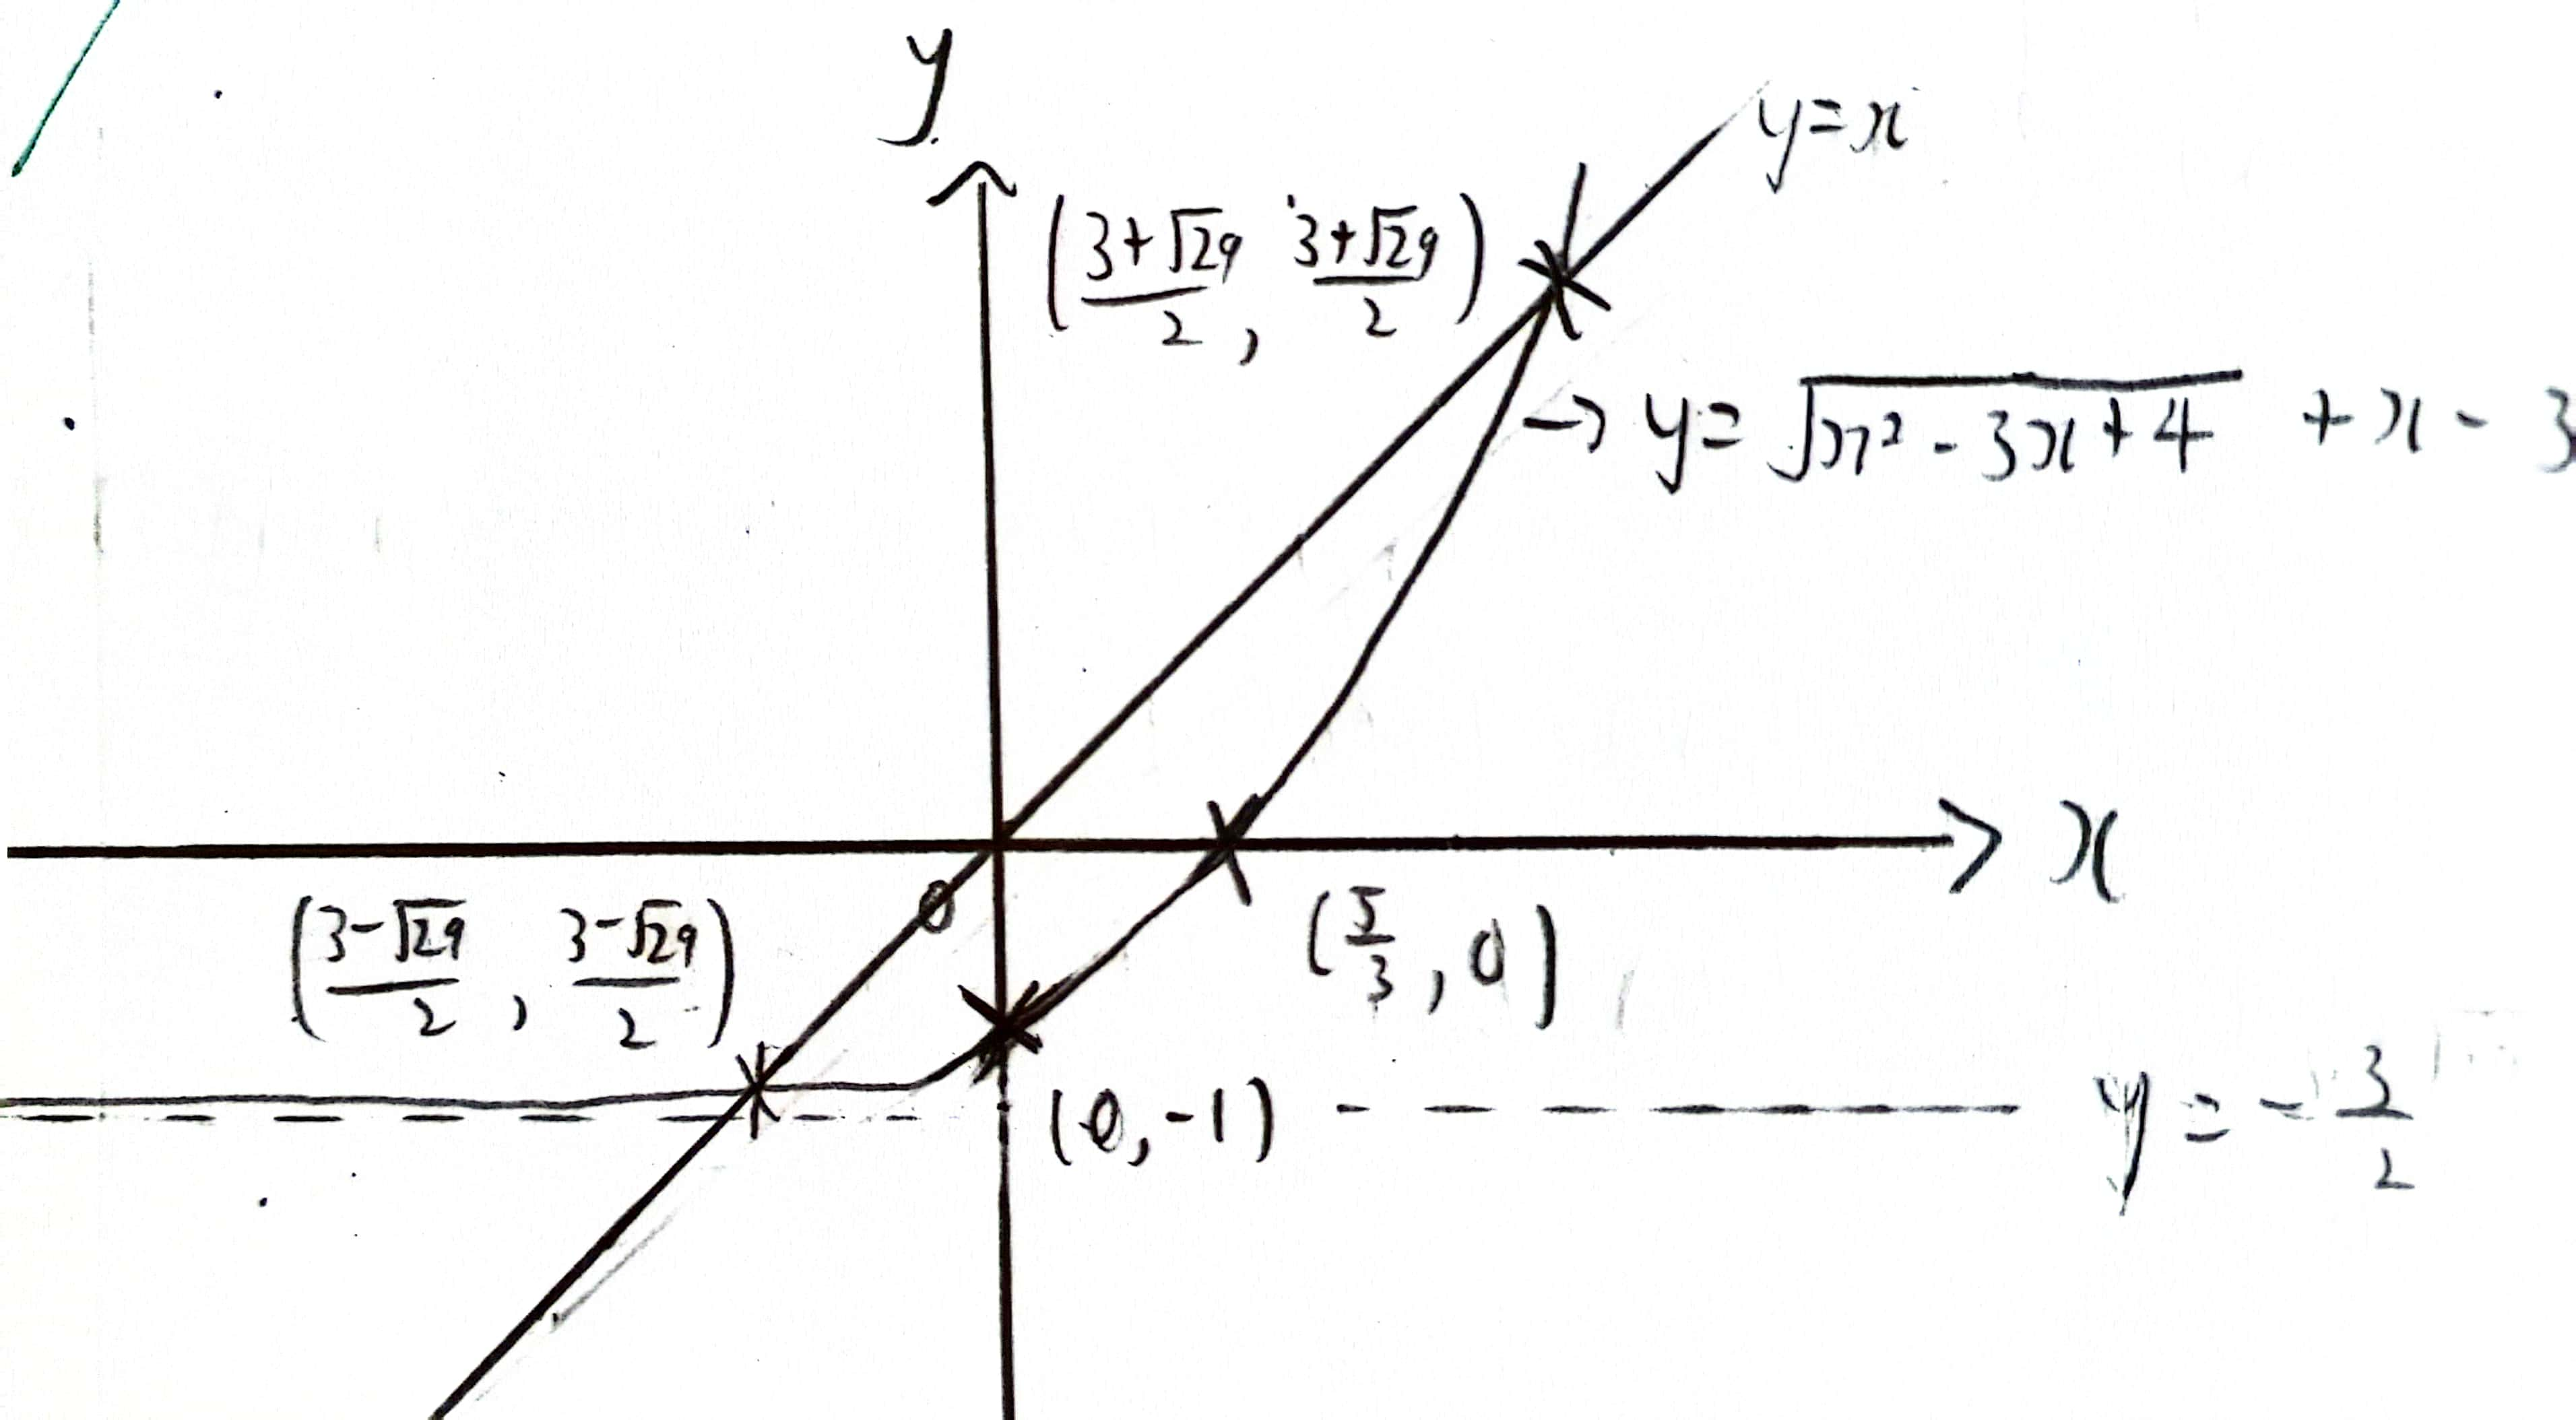
\includegraphics[scale=0.05]{SpecialRR.jpg}
    \captionof{figure}{The RR \(x_{n+1}=\sqrt{x_n^2-3x_n+4}+x_n-3\).}
  \end{center}
  Let \(f(x)=\sqrt{x^2-3x+4}+x-3\).
  \begin{enumerate}
    \item Suppose \(x_1 \leq \frac{3+\sqrt{29}}{2}\). For \(x_1<\frac{3-\sqrt{29}}{2}\), we see that \(f(x)>x\). So \(x_n\) increases till \(\frac{3-\sqrt{29}}{2}\). While for \(\frac{3-\sqrt{29}}{2}<x_1<\frac{3+\sqrt{29}}{2}\), we have \(f(x)<x\). Thus \(x_n\) decreases till \(\frac{3-\sqrt{29}}{2}\). Notice the graphs intersects at \(x=\frac{3-\sqrt{29}}{2}\). So, when \(x_n=\frac{3-\sqrt{29}}{2}\), if ever, then \(x_{n+1}=x_n\). That is, \(L=\frac{3-\sqrt{29}}{2}\).
    \item Similarly, if \(x_1=\frac{3+\sqrt{29}}{2}\), then \(x_n=\frac{3+\sqrt{29}}{2}\) is a constant function; \(L=\frac{3+\sqrt{29}}{2}\).
    \item Presume that \(x_n>\frac{3+\sqrt{29}}{2}\). Then, \(f(x)>x\) tells us \(x_n\) is an increasing sequence that is unbounded. In other words, \(L\) does not exist.
  \end{enumerate}
\end{example}

\chapter{Induction}
\begin{stbox}{General Information}
  Let \(P(x)\) be the statement that ``\ldots''.\\[3mm] 
  When \(n=1\), \ldots\\[3mm]
  \(\implies P(1)\) is true.\\[3mm]
  Assume \(P(k)\) is true for some \(k \in \mathbb{Z}^{+}\).\\[3mm]
  Then, \ldots\\[3mm]
  \(\implies P(k+1)\) is true.\\[3mm]
  Therefore, since \(P(1)\) is true and \(P(k)\text{ true}\implies P(k+1)\text{ true}\), \(P(n)\) is true for all \(n \in \mathbb{Z}^{+}\).
\end{stbox}

\chapter{Differentiation}
\begin{definition*}{}{}
  \begin{enumerate}
    \item A function \(f\) is called (strictly) increasing on an interval \(I\) iff \(f'(x)>0\) for all \(x \in I\).
    \item A function \(f\) is called monotonically increasing on an interval \(I\) iff \(f'(x) \geq 0\) for any \(x \in I\).
  \end{enumerate}
\end{definition*}
\begin{stbox}{General Information}
  \begin{enumerate}
    \item How to sketch the graph of the integral or derivative of a function \(f\).
    \item Relationship btw. a function \(f\) and its derivative, \(f'\):\\
    \begin{tabular}{|c|c|}
      \hline
      \(y=f(x)\) & \(y=f'(x)\)\\
      \hline
      Vertical asymptote at \(x=a\) & Vertical asymptote at \(x=a\).\\
      \hline
      Horizontal asymptote at \(y=a\) & Horizontal asymptote \(y=0\).\\
      \hline
    \end{tabular}
    \item Recap:\\
    \begin{tabular}{|Sc|Sc|}
      \hline
      \(f(x)\) & \(f'(x)\)\\
      \hline
      \(\sin^{-1}\left(\frac{x}{a}\right)\) & \(\frac{1}{\sqrt{a^2-x^2}}\), \(\lvert x \rvert<a\)\\
      \hline
      \(\cos^{-1}\left(\frac{x}{a}\right)\) & \(-\frac{1}{\sqrt{a^2-x^2}}\), \(\lvert x \rvert<a\)\\
      \hline
      \(\tan^{-1}\left(\frac{x}{a}\right)\) & \(\frac{a}{a+x^2}\), \(x \in \mathbb{R}\)\\
      \hline
      \(\log_a(f(x))\) &  \(\frac{1}{x \ln(a)}\)\\
      \hline
      \(a^x\) & \(a^x \ln(a)\)\\
      \hline
    \end{tabular}
    \item Implicit differentiation: \(\frac{dz}{dx}=\frac{dz}{dy}\cdot \frac{dy}{dx}\). \(\bigstar\) Makes life much easier (e.g. finding \(f^{(n)}(x)\)). 
    \item Parametric Differentiation: \(\frac{dy}{dx}=\frac{dy}{dt}\cdot \frac{dt}{dx}\).
    \item Small angle approximation: 
    \begin{enumerate}
      \item \(\sin(x) \approx x\),
      \item \(\cos(x) \approx 1-\frac{x^2}{2}\),
      \item \(\tan(x) \approx x\).
    \end{enumerate}
    \item Maclaurin Series: \(f(x)=\sum_{n=0}^{\infty}\frac{f^{(n)}(0)}{n!}x\).
  \end{enumerate}
\end{stbox}
\chapter{Integration Techniques}
\section{Basic Integration (IBS, IBP, etc)}
\begin{stbox}{General Information}
  \begin{enumerate}
    \item Factor Formulae \(\bigstar\) (must \emph{rmb}):
    \begin{enumerate}
      \item \(\sin(mx)\cos(nx)=\frac{1}{2}[\sin((m+n)x)+\sin((m-n)x)]\),
      \item \(\cos(mx)\cos(nx)=\frac{1}{2}[\cos((m+n)x)+\cos(m-n)x]\),
      \item \(\sin(mx)\sin(nx)=-\frac{1}{2}[\cos((m+n)x)-\cos((m-n)x)]\).
    \end{enumerate}
    \item Common classes of integrals:
    \begin{enumerate}
      \item Apply partial fractions:
      \[\int\frac{f(x)}{g(x)}\,dx.\]
      \item Split \(px+q\), then complete the square:
      \[\int \frac{px+1}{\sqrt{ax^2+bx+c}}\,dx \quad\text{or}\quad \int \frac{px+1}{ax^2+bx+c}\,dx\] 
    \end{enumerate}
    \item Integration by Substitution: 
    \[\int f(x) \, dx=\int f(x)\frac{dx}{du}\,du.\]
    \item Use Pythagoras' Theorem / draw a right-angled triangle to help with trig conversions, e.g.: \(\tan(\theta)\) to \(\frac{x+1}{\sqrt{2-(x+1)^2}}\).
    \item Integration by Parts:
    \begin{center}
      \begin{tabular}{ScSc}
        \(\begin{aligned}
          \text{Let }&u=g(x)\text{, }\frac{dv}{dx}=h(x),\\
          \frac{du}{dx}&=g'(x)\text{, }v=\int h(x)\, dx.
        \end{aligned}\) & \hspace{1cm}\(\begin{aligned}
          \int u\left(\frac{dv}{dx}\right)\,dx=uv-\int v \left(\frac{du}{dx}\right)\,dx.
        \end{aligned}\)
      \end{tabular}
    \end{center}
  \end{enumerate}
\end{stbox}
\newpage
\section{Areas \& Volumes}
\begin{stbox}{General Information}
  \begin{enumerate}
    \item Volume of revolution when rotated about \(x\)-axis: 
  \begin{enumerate}
    \item The disc method
    \[\int_{x_1}^{x_2}\pi y^2\,dx=\int_{x=x_1}^{x=x_1}\pi y^2\, \frac{dx}{dt}\,dt.\]
    \item The shell method:
    \[\int_{x_1}^{x_2}2\pi yx \,dy.\]
  \end{enumerate}
  \item Arc length:
  \begin{equation*}
    \resizebox{0.9\hsize}{!}{\(\displaystyle\int_{x_1}^{x_2}\sqrt{\left(\frac{dy}{dx}\right)^2+1}\,dx=\int_{y_1}^{y_2} \sqrt{\left(\frac{dx}{dy}\right)^2+1}\,dy=\int_{t_1}^{t_2}\sqrt{\left(\frac{dy}{dt}\right)^2+\left(\frac{dx}{dt}\right)^2}\,dt=\int_{\alpha}^{\beta}\sqrt{r^2+\left(\frac{dr}{d\theta}\right)^2}\,d\theta.\)}
    \end{equation*}
  \item Surface area of revolution when rotated about \(\highlight[blue!30]{x}\)-axis: 
  \begin{equation*}
    \resizebox{0.9\hsize}{!}{\(\displaystyle\int_{x_1}^{x_2}2\pi \highlight[red!30]{y} \sqrt{\left(\frac{dy}{dx}\right)^2+1}\,dx=\int_{y_1}^{y_2}2\pi \highlight[red!30]{y} \sqrt{\left(\frac{dx}{dy}\right)^2+1}\,dy=\int_{t_1}^{t_2}2\pi \highlight[red!30]{y} \sqrt{\left(\frac{dy}{dt}\right)^2+\left(\frac{dx}{dt}\right)^2}\,dx=\int_{\alpha}^{\beta}\frac{1}{2}r^2\,d\theta.\)}
    \end{equation*}
  \begin{flushleft}
    \(\bigstar\) Rotating about \(\highlight[blue!30]{x}\)-axis \(\implies\) \(\highlight[red!30]{y}\) in integrand\\
    \hphantom{\(\bigstar\)} Rotating about \(\highlight[blue!30]{y}\)-axis \(\implies\) \(\highlight[red!30]{x}\) in integrand.
  \end{flushleft}
  \end{enumerate}
\end{stbox}
\newpage
\section{Numerical Methods}
\subsection{Trapezium Rule}
\begin{stbox}{General Information}
    \begin{enumerate}
      \item Formula for \(n\) intervals, or (n+1)ordinates, of width \(h:=(b-a)/n\): 
      \[\int_{a}^{b}y\,dx=\frac{h}{2}(y_0+2y_1+2y_2+\cdots+2y_{n-1}+y_n).\]
      \item Illustration
      \begin{center}
        \includestandalone{../Diagrams/Trapezium}
        \captionof{figure}{Trapezium rule}
      \end{center}
    \item Error: 
    \begin{enumerate}
      \item Concave upwards, i.e. (\(f'(x)\) is increasing / \(f''(x)>0\)) \(\implies\) overestimation.
      \item Concave downwards, i.e. (\(f'(x)\) is decreasing / \(f''(x)<0\)) \(\implies\) underestimation.
    \end{enumerate}
    \end{enumerate}
    \end{stbox}
    \newpage
    \subsection{Simpson's Rule}
    \begin{stbox}{General Information}
      \begin{enumerate}
        \item Formula for \(n\) intervals, or (n+1)ordinates, of width \(h:=(b-a)/n\):
        \[\int_{a}^{b}y\,dx=\frac{h}{3}(y_0+4y_1+2y_2+4y_3+\cdots+2y_{n-2}+4y_{n-1}+y_n).\]
        Note that the number of intervals \(n\) should be \emph{even}, that of ordinates \emph{odd}.
        \item Illustration
        \begin{center}
          \includestandalone{../Diagrams/Simpson}
          \captionof{figure}{Simpson's rule}
        \end{center}
      \end{enumerate}
    \end{stbox}
      \begin{note}
        Accuracy of the Trapezium rule vs Simpson's Rule:
        ``Simpson's Rule uses \emph{quadratic curves} to interpolate the points on the curve so it usually \emph{gives a better approximation} to the actual curve than the trapezium rule which uses \emph{straight lines} to interpolate the ordinates.''
      \end{note}
  \chapter{Complex Numbers}
  \section{Complex Number I}
  \begin{stbox}{General Information}
    \begin{enumerate}
      \item Find the square root of \(x+iy\): Let \(\sqrt{x+iy}=a+bi\). Then square both sides \& solve.
      \item Simplifying fractions: multiply by the denominator's conjugate
      \[\frac{a+bi}{c+di}=\frac{a+bi}{c+di}\cdot\frac{c-di}{c-di}=\cdots.\]
      \item Polynomials:
      \begin{enumerate}
        \item Fundamental Theorem of Algebra: If \(p(z):=\sum_{i=0}^{n}a_iz^i\) is a polynomial of degree \(n \geq 1\) with complex coefficients, then there exists complex numbers \(c_i\) for each \(1 \leq i \leq n\) such that 
        \[p(z)=a_n \prod_{i=1}^{n}(z-c_i).\]
        \item If a polynomial in real coefficients only has root \(a+bi\), then \(a-bi\) is another root.
      \end{enumerate}
    \end{enumerate}
    \end{stbox}
        \begin{example}{}{}
          Find the roots of \(iz^2+2z+3i=0\).
          \begin{align*}
            z^2-2iz+3&=0\\
            z&=\frac{2i \pm \sqrt{(2i)^2-4(1)(3)}}{2(1)}=i \pm \frac{\sqrt{-16}}{2}=i \pm 2i
          \end{align*}
          So, \(z=3i\) or \(z=-i\).
        \end{example}
        \begin{example}{N2010/2/1}{}
          One root of the equation \(x^4+4x^3+ax+b=0\), where \(a\) and \(b\) are real, is \(x=-2+i\). Find the values of \(a\) and \(b\) and the other roots.\\[3mm]
          Substitute \(-2+i\) into the equation:
          \begin{align*}
            (-2+i)^4+4(-2+i)^3+(-2+i)^2+a(-2+i)+b&=0\\
            -12+16i&=2a-b-ai\\
            a=-16, &\hphantom{=}\ \ 2a-b=-12
          \end{align*}
          Therefore, \(a=-16\), \(b=-20\).\\[3mm]
          \emph{Since all the coefficients of the polynomial are real} (\textbf{explain}), \(-2-i\) is another root. Now, \(x^4+4x^3+ax+b=(x-(-2+i))(x-(-2-i))(cx+d)\) for some \(c,d \in \mathbb{R}\).\\[3mm]
          Accordingly, substitute \(x=0\), then \(x=2\), and solve. Alternatively, notice \(x^4+4x^3+ax+b=(x^2-2(-2)x+((-2)^2+1^2))(x^2+cx+d)=(x^2+4x+5)(x^2+4x+5)\). Either ways, we have \(c=0\) and \(d=-4\). As such, the last two roots are \(x=-2 \pm i\) and \(x=\pm 2\). 
        \end{example}
      \begin{stbox}{}
        \begin{itemize}[label=\hphantom{1.}]
          \item
          \begin{enumerate}[label=(\alph*)]
            \setcounter{enumi}{2}
            \item Simultaneous equations: Solve as usual.
            \item Properties of modulus: \(\lvert z_1^xz_2^y \rvert=\lvert z_1 \rvert^x \lvert z_2 \rvert^y\), for any \(x,y \in \mathbb{R}\).
            \item Properties of arguments (same as \(\log\)): \(\arg(z) \in (-\pi,\pi]\) and \(\arg(z_1^xz_2^y)=n\arg(z_1)+m\arg(z_2)\) for any \(x,y \in \mathbb{R}\).
            \item Polar form: \(z=re^{i\theta}\).
            \item Polar/Trigonometric form: \(z=r[\cos(\theta)+i\sin(\theta)]\).
          \end{enumerate}
        \end{itemize}
  \end{stbox}
  \begin{note}
    Show that the value of \(w^n\) is either \(2^n\) or \(2^{-n}\) for integers \(n\).\\[3mm]
    Then we \textbf{must} show that \(w^n=\cdots=\begin{cases}
      2^n(1)=2^n&\text{if }n\text{ even},\\
      2^n(-1)=-2^n&\text{if }n\text{ odd}.
    \end{cases}\) 
  \end{note}
\section{Complex Numbers II}
\begin{theorem}{De Moivre's Theorem}{}
  Let \(z\) be a complex number, \(n\) an integer, and \(\theta\) an angle. Suppose \(z=re^{i\theta}\). Then, 
  \[z^n=e^{i\theta}=r^n[\cos(n\theta)+i\sin{n\theta}].\]
\end{theorem}
\begin{stbox}{General Information}
  \begin{enumerate}
    \item All \(n\)th roots of any complex number are the same distance \(r\) from the origin and have the same angular separation, \(\pi/n\).
    \item Note that \(1+e^{i\theta}=e^{i\theta/2}(e^{-i\theta/2}+e^{i\theta/2})\).
    \item For \(z=re^{i\theta}\), we have \(z^n+z^{-n}=2\cos(n\theta)\) and \(z^n-z^{-n}=2i\sin(n\theta)\).
    \item The geometric meaning of multiplying by \(i\) is a anti-clockwise rotation by \(\pi\) radians.
    \item Loci (Use a \emph{compass})
    \begin{enumerate}
      \item The locus represented by \(\lvert z-a \rvert =r\) (or \(z=a+re^{i\theta}\)) is a \emph{circle} of radius \(r\) centered at \(A(x,y)\) (where \(a:=x+iy\)).
      \begin{center}
        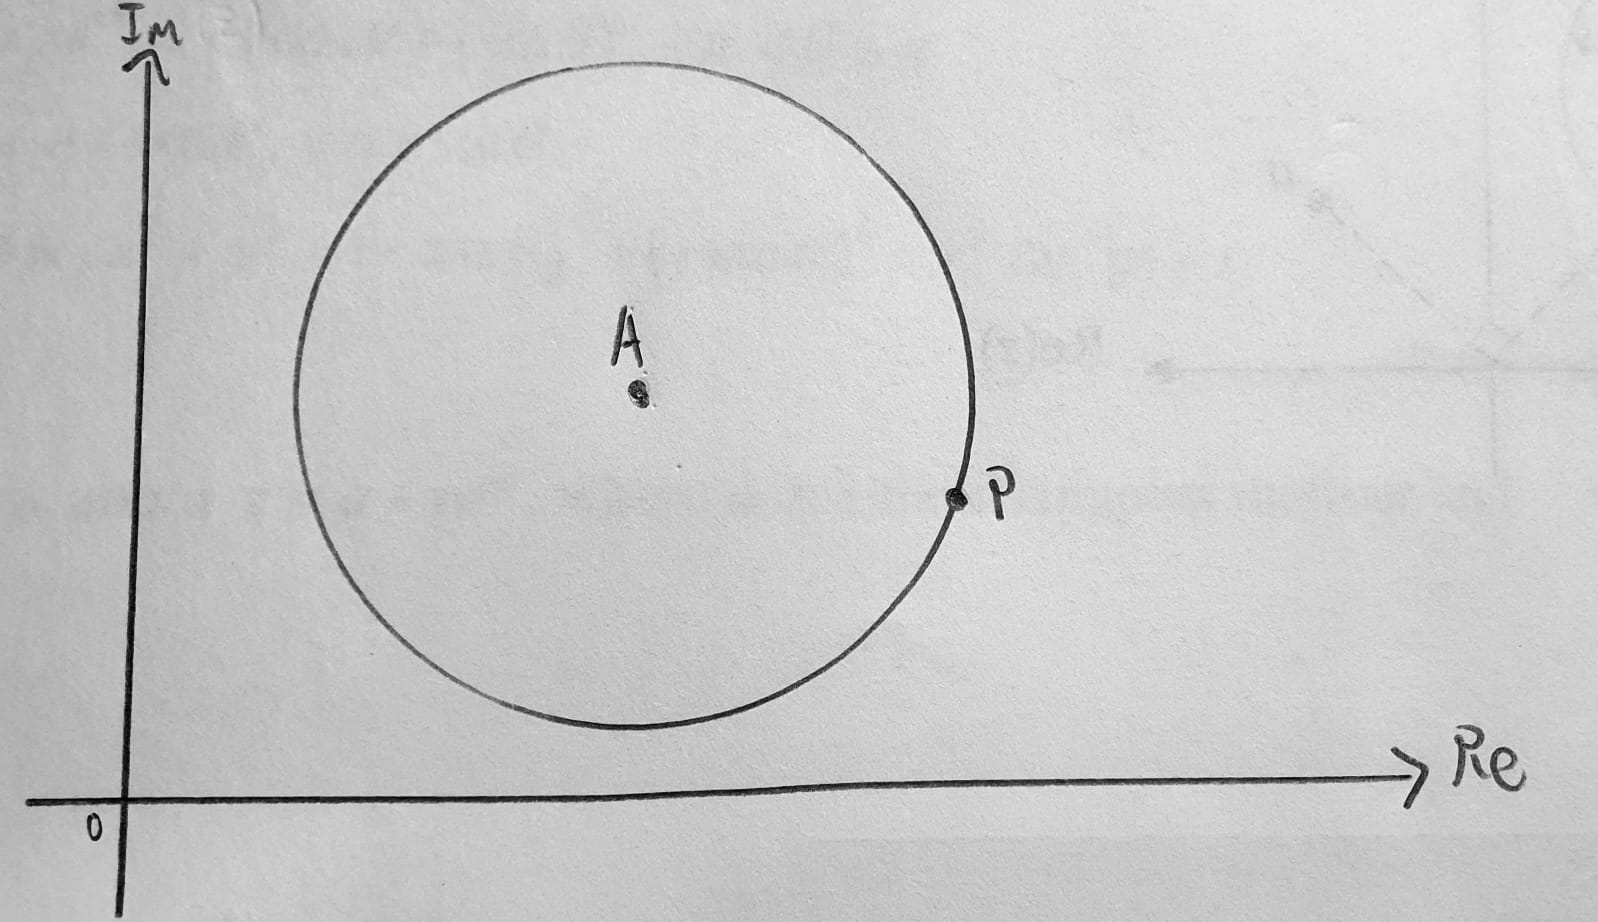
\includegraphics[scale=0.1]{../images/ComplexCircleLocus}
        \captionof{figure}{The locus of \(\lvert z-a \rvert =r\).}
      \end{center}
      \begin{enumerate}
        \item Either label the four points to the direct North, South, East, West of the circle, or denote the radius clearly. 
        \item The line segment, representing the furthest distance from a point to a circle, always cuts through the circle's centre. So, the distance
        \[\text{OP}_{\text{max}}-\text{OP}_{\text{min}}=2\cdot\text{radius}.\]
        \item The line segments, from a point to a circle that produces the largest angle, are tangents to the circle.
        \begin{center}
          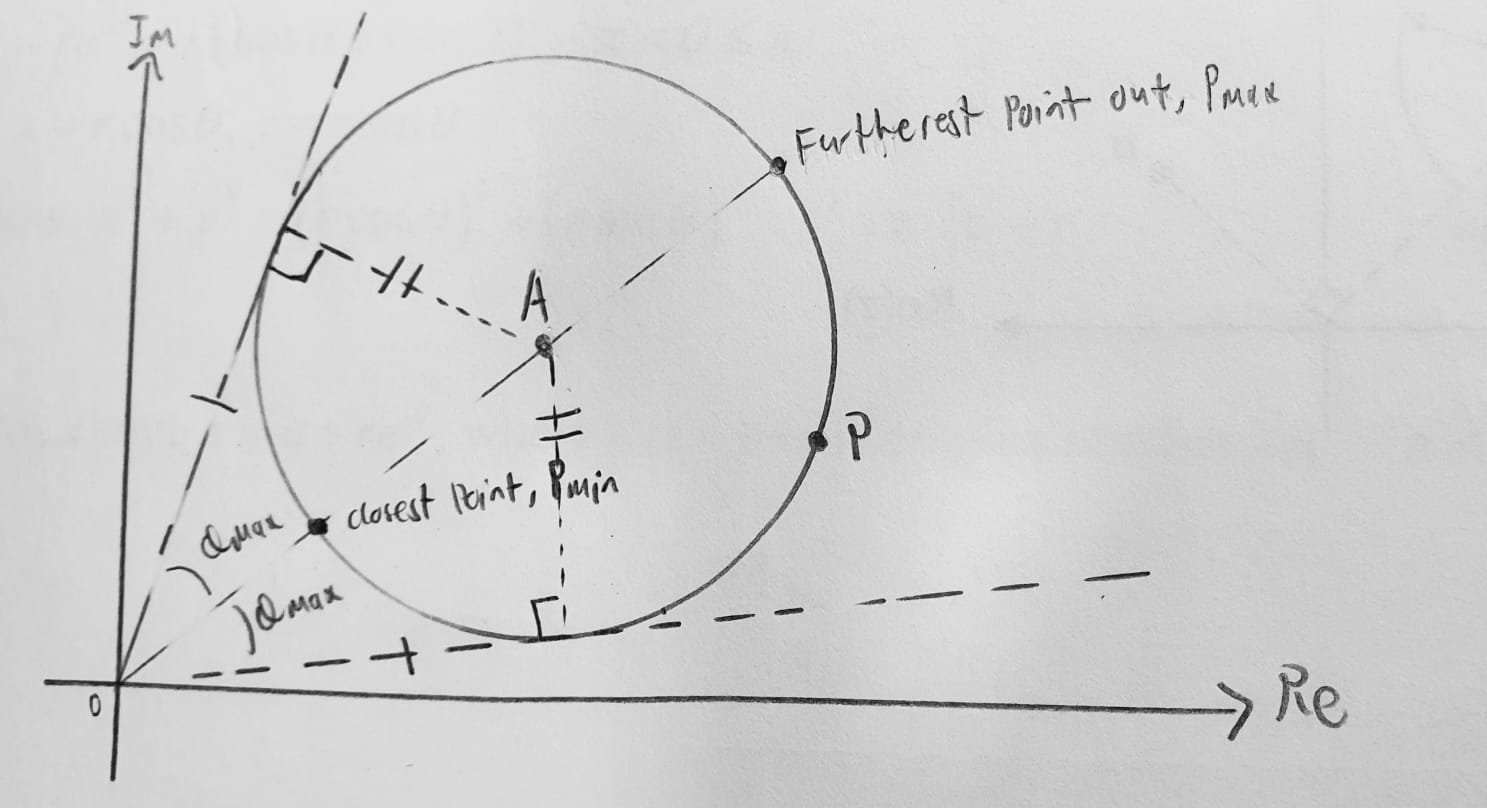
\includegraphics[scale=0.15]{ComplexLocusCircle-LargestAngleAndDistance.jpg}
          \captionof{figure}{Maxmium distance and angle of a point from a circle}
        \end{center}
      \end{enumerate}
      \newpage
      \item The locus represented by \(\lvert z-a \rvert =\lvert z-b \rvert\) is the \emph{perpendicular bisector} of the line segment joining \(A\) and \(B\).
      \begin{center}
        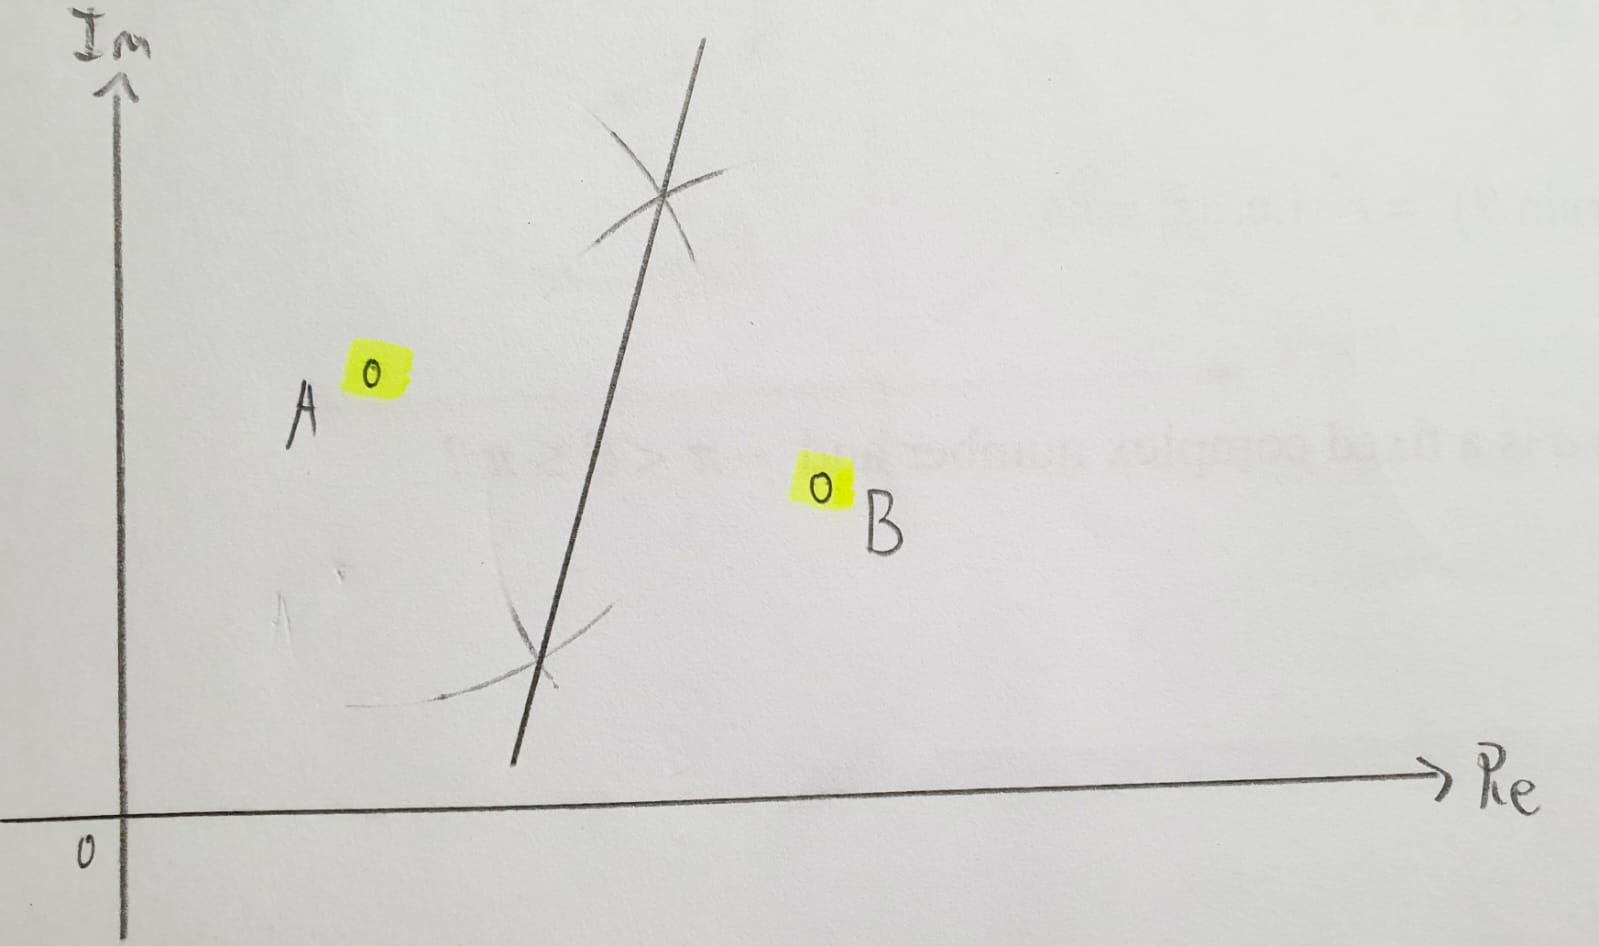
\includegraphics[scale=0.12]{../images/ComplexPerpendicularBisectorLocus}
        \captionof{figure}{The locus of \(\lvert z-a \rvert =\lvert z-b \rvert\), a perpendicular bisector}
      \end{center}
      \item The locus represented by \(\arg(z-a)=\theta\) is the \emph{half-line} from \(A\) (excluding \(A\)) that makes an angle \(\theta\) with the \emph{positive} real axis.
      \begin{center}
        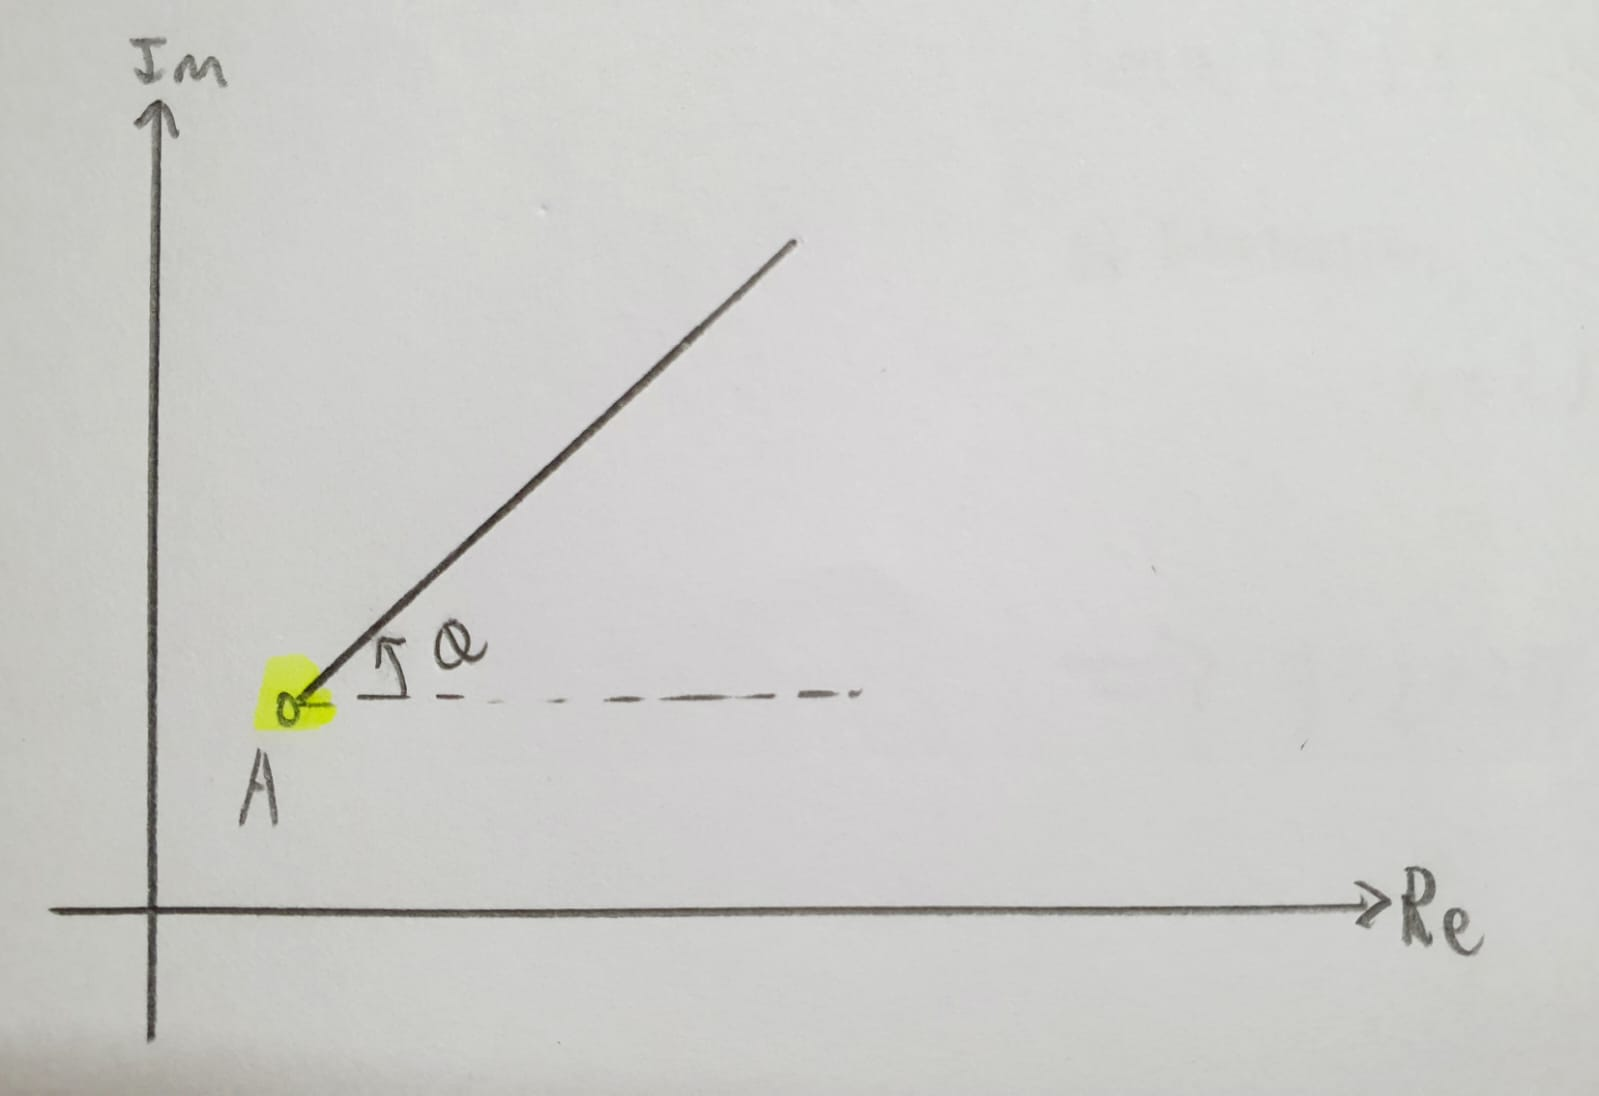
\includegraphics[scale=0.1]{../images/ComplexRotationByAngleTheta}
        \captionof{figure}{The locus of \(\arg(z-a)=\theta\), a half-line.}
      \end{center}
    \end{enumerate}
    \item There is no need to find the points of intersection between two loci, unless the questions states so. 
  \end{enumerate}
\end{stbox}
\begin{example}{TQ 10(b)}{}
  Show that \(\cot^2(2\pi/5)\) is a root of the equation \(px^2+qx+r=0\), where we are given 
  \[\cot(4\theta)=\frac{\cot^4(\theta)-6\cot^2(\theta)+1}{4\cot^3(\theta)-4\cot(\theta)}.\]
  First notice that \(\cot(8\pi/5)=-\cot(2\pi/5)\). So, 
  \[-\cot(2\pi/5)=\frac{\cot^4(2\pi/5)-6\cot^2(2\pi/5)+1}{4\cot^3(2\pi/5)-4\cot(2\pi/5)}.\]
  Simplifying gives 
  \[5[\cot^2(2\pi/5)]^2-10[\cot^2(2\pi/5)]+1=0.\]
  Thus, \(x=cot^2(2\pi/5)\) is a root of the equation \(5x^2-10x+1=0\). 
\end{example}

\subfile{Subfiles/FMAsubfile.tex}

\chapter{Graphing Techniques}
\section{Graphing `Familiar' Functions and Asymptotic bois}

\begin{definition*}{}{}
  \begin{enumerate}
    \item \textbf{Lines of Symmetry}: A \emph{line of symmetry} of a function is a line, such that the function is a reflection of itself about that line.
    \item \textbf{Horizontal Asymptotes}: A (horizontal) line \(g(x)=c\) is the \emph{horizontal asymptote} of the curve \(f(x)\) iff \(\lim_{x \to \infty}{f(x)}=c\) (or with \(-\infty\) instead of \(\infty\)).\footnote{Otherwise notated by \(f(x) \to c\) as \(x \to \infty\).}
    \item \textbf{Vertical Asymptotes}: A (vertical) line \(x=c\) is a \emph{vertical asymptote} of the curve \(f(x)\) iff \(\lim_{x \to c}{f(x)}=\operatorname{\infty} \text{ or } -\infty\).
    \item \textbf{Oblique Asymptotes}: A line \(g(x)=mx+c\) --- where \(m \neq 0\) --- is an \emph{oblique asymptote} of the curve \(f(x)\) iff \(\lim_{x \to \infty}[f(x)-g(x)]=0\) (or with \(-\infty\) instead of \(\infty\)).
\end{enumerate}
\end{definition*}
\begin{stbox}{Curve Sketching of Rational Functions}
  \begin{enumerate}
    \item[\textbf{S}] Stationary points
    \item[\textbf{I}] Intersection with axes
    \item[\textbf{A}] Asymptotes   
  \end{enumerate}
  \begin{enumerate}[label=\roman*]
    \item Know how to sketch the graphs of \(y=\frac{ax+b}{cx+d}\) and \(y=\frac{ax^2+bx+c}{dx+e}\).
    \item Rectangular Hyperbolas \(\left(\text{of the form \(y=\frac{ax+b}{cx+d}\)}\right)\):
    \begin{itemize}
      \item \emph{Two} asymptotes, namely \(x=-\frac{d}{c}\) and \(y=\frac{a}{c}\).
      \item \emph{Two} lines of symmetry with gradients \(\pm 1\) \emph{and} pass through the intersection point of the aforementioned two asymptotes.
    \end{itemize}
    \item \emph{If} \(n=\operatorname{deg}P=\operatorname{deg}Q\), then
    \begin{itemize}
      \item \(y=R(x)\) is the \emph{horizontal} asymptote of \(\frac{P(x)}{Q(x)}=R(x)+\frac{S(x)}{Q(x)}\).
      \item Equivalently, \(y=\frac{\operatorname{coeff}_P(x^n)}{\operatorname{coeff}_Q(x^n)}\) is a \emph{horizontal} asymptote.\footnote{E.g.: \(y=\frac{1}{15}\) is a horizontal asymptote of \(y=\frac{\text{\hly{\(1\)}}x^2+2x-3}{(\text{\hly{\(5\)}}x+1)(\text{\hly{\(3\)}}x+2)}\).}
    \end{itemize}
    \item If \(\operatorname{deg}P=\operatorname{deg}Q+1\), then \(R(x)\) is an \emph{oblique} asymptote of \(\frac{P(x)}{Q(x)}=R(x)+\frac{S(x)}{Q(x)}\).
    \item Write down asymptotes and lines of symmetry.\footnote{E.g.: \begin{itemize}
      \item[] Asymptotes: \(x=4\), \(y=20\).
      \item[] Lines of Symmetry: \(y=x+16\), \(y=-x+24\).
    \end{itemize} } If none are present indicate with ``No lines of symmetry.''
  \end{enumerate}
\end{stbox}
\begin{IN}
  \begin{itemize}
    \item The discriminant can be very useful.
    \item Know how to use the G.C. Transfrm app.
    It allows you to vary the value of some parameter \(A\) for a function \(f(Ax)\). Use this to graphically find the values of integer \(k\) satisfying some conditions.
  \end{itemize}
\end{IN}

\section{Conics}
``Tikz is pain, PGFPlots is suffering'' --- Wise Man.
\begin{center}
  \small
  \begin{tabular}{|c|c|c|}
    \hline
    & Ellipses & Hyperbolas\\
    \hline
    Standard Forms & \(\frac{(x-h)^2}{a^2}+\frac{(y-k)^2}{b^2}=1\) & 
    \begin{tabular}{@{}c@{}} 
     \\
    \(\frac{(x-h)^2}{a^2}-\frac{(y-k)^2}{b^2}=1\)\\
    \(\frac{(y-k)^2}{b^2}-\frac{(x-h)^2}{a^2}=1\)\\
    \\
    \end{tabular}\\
    \hline
    General Equation & 
    \begin{tabular}{@{}c@{}} 
      \(ax^2+by^2+cx^2+dx+e=0\),\\
      \footnotesize where \(\operatorname{sgn}(a)=\operatorname{sgn}b\). \normalsize
     \end{tabular}
     &
     \begin{tabular}{@{}c@{}} 
      \(ax^2+by^2+cx^2+dex+e=0\),\\
      \footnotesize where \(\operatorname{sgn}(a) \neq \operatorname{sgn}b\). \normalsize
     \end{tabular}\\
     \hline
     Center & \multicolumn{2}{c|}{\((h,k)\)}\\
    \hline
    \begin{tabular}{@{}c@{}} 
      Vertical `Radius'\\
      \footnotesize (variables here from \emph{standard form}!) \normalsize
    \end{tabular}
      & \multicolumn{2}{c|}{\(b\)}\\
      \hline
    \begin{tabular}{@{}c@{}} 
        Horizontal `Radius'\\
        \footnotesize (variables here from \emph{standard form}!) \normalsize
    \end{tabular}
    & \multicolumn{2}{c|}{\(a\)}\\
    \hline
    \begin{tabular}{@{}c@{}} 
      Vertical  Vertices\\
      \footnotesize (variables here from \emph{standard form}!) \normalsize
    \end{tabular}
    & \multicolumn{2}{c|}{\((h, k \pm b)\)}\\
    \hline
    \begin{tabular}{@{}c@{}} 
      Horizontal Vertices\\
      \footnotesize (variables here from \emph{standard form}!) \normalsize
    \end{tabular}
    & \multicolumn{2}{c|}{\((h \pm a,k)\)}\\
    \hline
    Shape & 
    \begin{tikzpicture}[scale=0.5]
      
      \begin{axis}[axis lines=middle,axis line style =-{Classical TikZ Rightarrow[length=5pt 3 0]},every axis x label/.style = {%
        at = {(xticklabel cs:1.05)},
        anchor = north},
      every axis y label/.style = {%
        at = {(yticklabel cs:1.05)},
        anchor=east},
        xtick=\empty, ytick=\empty,clip=false,xmin=0,xmax=11,xlabel=\Large\(x\),ylabel=\Large\(y\),ymin=0,ymax=6
        ]
        
      \draw[blue] (5,3) ellipse (5 and 2);
    
      % label center
      \node at (5,3) [below right] {\Large \((h,k)\)};

      \node at (5,3) {\Large \color{red}{\(\times\)}};
    
      % draw h-line
      \draw[->,arrows = -{Classical TikZ Rightarrow[length=5pt 3 0]}] (5,3) -- (0,3) node[midway, above] {\Large \(a\)};
    
      % draw another h-line
      \draw[->,arrows = -{Classical TikZ Rightarrow[length=5pt 3 0]}] (5,3) -- (10,3);
    
      % draw k-line
      \draw[->,arrows = -{Classical TikZ Rightarrow[length=5pt 3 0]}] (5,3) -- (5,5) node[midway, right] {\Large \(b\)};
    
      % draw another k-line
      \draw[->,arrows = -{Classical TikZ Rightarrow[length=5pt 3 0]}] (5,3) -- (5,1);

      \addplot+[
  mark=x,
  only marks,
  mark size=6pt,
  mark options={line width=1.5pt,red}
] 
  coordinates
  {(5,3)};
  
      \end{axis}
      % draw ellipse
      \addvmargin{3mm}
    \end{tikzpicture} & 
    \begin{tabular}{@{}c@{}} 
      \(\operatorname{coeff}(x^2)<0\)\\
      \begin{tikzpicture}[scale=0.5]
      
        \begin{axis}[axis lines=middle,axis line style =-{Classical TikZ Rightarrow[length=5pt 3 0]},every axis x label/.style = {%
          at = {(xticklabel cs:1.05)},
          anchor = north},
        every axis y label/.style = {%
          at = {(yticklabel cs:1.05)},
          anchor=east},
          xtick=\empty, ytick=\empty,clip=false,xmin=-1,xmax=11,xlabel=\Large\(x\),ylabel=\Large\(y\),ymin=-1,ymax=7
          ]
          
      \addplot [red,thick,domain=-2:2] ({sinh(x)+5}, {cosh(x)+3});
      \addplot [red,thick,domain=-2:2] ({-sinh(x)+5}, {-cosh(x)+3});
      \addplot[red,dashed,domain=1:9] {x-2};
      \addplot[red,dashed,domain=1:9] {-x+8};

        \node at (5,3) [below] {\Large \((h,k)\)};
  
        \node at (5,3) {\LARGE  \color{blue}{\(\times\)}};
      
        % draw h-line
        \draw[->,arrows = -{Classical TikZ Rightarrow[length=3pt 3 0]}] (5,4) -- (4,4) node[midway, above] {\Large \(a\)};
      
        % draw k-line
        \draw[->,arrows = -{Classical TikZ Rightarrow[length=3pt 3 0]}] (5,3) -- (5,4) node[midway, right] {\Large \(b\)};
        
        \addplot+[
  mark=x,
  only marks,
  mark size=6pt,
  mark options={line width=1.5pt}
] 
  coordinates
  {(5,3)};

        \end{axis}
        % draw ellipse
      \end{tikzpicture}\\
      \(\operatorname{coeff}(y^2)<0\)\\
      \begin{tikzpicture}[scale=0.5]
      
        \begin{axis}[axis lines=middle,axis line style =-{Classical TikZ Rightarrow[length=5pt 3 0]},every axis x label/.style = {%
          at = {(xticklabel cs:1.05)},
          anchor = north},
        every axis y label/.style = {%
          at = {(yticklabel cs:1.05)},
          anchor=east},
          xtick=\empty, ytick=\empty,clip=false,xmin=-1,xmax=11,xlabel=\Large\(x\),ylabel=\Large\(y\),ymin=-1,ymax=7
          ]
          
        \addplot [red,thick,domain=-2:2] ({cosh(x)+5}, {sinh(x)+3});
      \addplot [red,thick,domain=-2:2] ({-cosh(x)+5}, {sinh(x)+3});
      \addplot[red,dashed,domain=1:9] {x-2};
      \addplot[red,dashed,domain=1:9] {-x+8};

        \node at (5,3) [below=0.25cm] {\Large \((h,k)\)};
  
        \node at (5,3) {\LARGE  \color{blue}{\(\times\)}};
      
        % draw h-line
        \draw[->,arrows = -{Classical TikZ Rightarrow[length=3pt 3 0]}] (5,3) -- (4,3) node[midway, above] {\Large \(a\)};
      
        % draw k-line
        \draw[->,arrows = -{Classical TikZ Rightarrow[length=3pt 3 0]}] (4,3) -- (4,4) node[midway, left] {\Large \(b\)};

        \addplot+[
  mark=x,
  only marks,
  mark size=6pt,
  mark options={line width=1.5pt}
] 
  coordinates
  {(5,3)};

        \end{axis}
        % draw ellipse
      \end{tikzpicture}
    \end{tabular}\\
    \hline
    \begin{tabular}{@{}c@{}} 
      Asymptotes\\
      (No need to rmb!)
    \end{tabular}
    & - & \(y=k \pm \frac{b(x-h)}{a}\)\\
    \hline
    Lines of Symmetry & \multicolumn{2}{c|}{\(x=h\), \(y=k\)}\\
    \hline
  \end{tabular}
  \normalsize
\end{center}
\begin{stbox}{General Information}
  \begin{itemize}
    \item To find asymptote of hyperbolas, just solve  
    \[\frac{(x-h)^2}{a^2}=\frac{(y-k)^2}{b^2}.\]
    \item Label vertices or radii, together with the center and asymptotes.
  \end{itemize}
\end{stbox}
\section{Parametric Equations}
\begin{IN}
  \begin{itemize}[label=\(\star\)]
    \item Check the qns for any \emph{restrictions} on the parameter! And modify that of the G.C.'s accordingly (Tmin \& Tmax).
    \item Vary the \(t\)-step or resolution (when using cartesian coordinates) when the graph is oddly jagged.
  \end{itemize}
\end{IN}
\section{Scaling, Translations, and Reflections}

\begin{center}
  \begin{tabular}{|Sc|Sc|Sc|}
    \hline
    \multicolumn{3}{|Sc|}{\large \color{blue}{Playing With \(x\)}}\\
    \hline
    Function & \(x\) is replaced with & (Horizontal) Transformation\\
    \hline 
    \(f(x+a)\) & \(x+a\) & 
    \begin{tabular}{@{}c@{}} 
      Translate \(a\) units in the positive (\(a \leq 1\))\\ 
      O/R negative \(x\)-direction (\(a \geq 1\)).
    \end{tabular}\\
    \hline 
    \(f(-x)\) & \(-x\) & Reflect about the \(y\)-axis\\
    \hline
    \(f(ax)\) & \(ax\) & Scale parallel to the \(x\)-axis by a scale factor of \(\frac{1}{a}\) if\footnote{otherwise simply reflect first} \(a \geq 1\).\\
    \hline
    \multicolumn{3}{|Sc|}{\large \color{red}{Playing With \(f(x)\)}}\\
    \hline
    \multicolumn{2}{|c|}{Function / Change to \(f(x)\)} & (Vertical) Transformation\\
    \hline
    \multicolumn{2}{|c|}{\(f(x)+a\)} & \begin{tabular}{@{}c@{}} 
      Translate \(a\) units in the positive (\(a \geq 1\))\\ 
      O/R negative \(y\)-direction (\(a \leq 1\)).
    \end{tabular}\\
    \hline
    \multicolumn{2}{|c|}{\(-f(x)\)} & Reflect about the \(x\)-axis.\\
    \hline
    \multicolumn{2}{|c|}{\(af(x)\)} & Scale parallel to the \(y\)-axis by scale factor \(a\).\\
    \hline
  \end{tabular}
\end{center}
\begin{IN}
\begin{center}
  \begin{tikzpicture}
    \node[ellipse, draw=blue, thick, minimum size=10mm,align=center] (x) at (1,0) {Transform \(x\)\\[2mm]
    Translation \ding{239} Scaling / Reflection};
    \node[ellipse, draw=red, thick, minimum size=10mm,align=center] (y) at (1,-3) {Transform \(y\)\\[2mm]
    Scaling / Reflection \ding{239} Translation};
    \draw [black, line width=0.75pt, arrows = {-Latex[open,scale=2]}] (x) to (y);
  \end{tikzpicture}
\end{center}
\end{IN}
\newpage
\section{\(\lvert f(x) \rvert\) and \(f( \lvert x \rvert)\)}
\begin{stbox}{General Information}
  \begin{itemize}
    \item For \(\lvert f(x) \rvert\), simply flip the part of the graph of \(f(x)\) that is below the \(x\)-axis, to above the \(x\)-axis.
    \item For \(f(\lvert x \rvert)\), its graph is symmetric about the \(x\)-axis
  \end{itemize}
\end{stbox}
\section{\(y=\frac{1}{f(x)}\)}
\begin{center}
  \begin{tabular}{|Sc|Sc|}
    \hline
    Behavior of \(f(x)\) & Behavior of \(1/f(x)\)\\
    \hline
    \(f(x)>0\) & \(\frac{1}{f(x)}>0\)\\
    \hline 
    \(f(x)<0\) & \(\frac{1}{f(x)}<0\)\\
    \hline
    Vertical Asymptote at \(x=c\) & \begin{tabular}{@{}c@{}} 
      \(\frac{1}{f(x)}\) \emph{tends} to 0\\
      \scriptsize \(^{*}\frac{1}{f(x)}\) is undefined at \(x=c\) \normalsize\\
    \end{tabular}\\
    \hline
    \multicolumn{2}{|Sc|}{\begin{tabular}{@{}c@{}} 
      \(\frac{df}{dx}=-\frac{d}{dx}\mathopen{}\left(\frac{1}{f(x)}\right)\)\\
      \scriptsize i.e. when \(f(x)\) increases, \(\frac{1}{f(x)}\) decreases. \normalsize\\
    \end{tabular}}\\
    \hline 
    \((a,b)\) is a \emph{minimum} pt & \(\left(a,\frac{1}{b}\right)\) is a \emph{maximum} pt\\
    \hline
    \((a,b)\) is a \emph{maximum} pt & \(\left(a,\frac{1}{b}\right)\) is a \emph{minimum} pt\\
    \hline
  \end{tabular}
\end{center}
\chapter{Polar Curves}
\begin{center}
  \begin{tikzpicture}
    %		%Grid
    %		\draw[thin, dotted] (0,0) grid (8,8);
    %		\foreach \i in {1,...,8}
    %		{
    %			\node at (\i,-2ex) {\i};	
    %		}
    %		\foreach \i in {1,...,8}
    %		{
    %			\node at (-2ex,\i) {\i};	
    %		}
    %		\node at (-2ex,-2ex) {0};
        
        %Coordinates		
        \coordinate (A) at (6,0);
        \coordinate (B) at (0,0);
        \coordinate (C) at (2.5,2.5);
        \coordinate (B') at (2.5,3.5);
        \coordinate (A') at (1.8,3.2);
        \coordinate (T) at (2.5,-2.5);
        \coordinate (G) at (-6,0);
        
        %Axis
        \draw[thick] (-2.5ex,0) -- (5,0) node [below] {\(\theta=0\)};
        \draw[thick] (0,-5) 
        node [left] {\(\theta=-\frac{\pi}{2}\)} 
        -- (0,5) 
        node [left] {\(\theta=\frac{\pi}{2}\)};
        
        %Vectors
        \draw[thick,blue] (0,0) -- (2.5,2.5) node[pos=0.6, above left] {\(r\)};
        \draw[thick,red] (0,0) -- (2.5,-2.5) node[pos=0.6, below left] {\(r\)};
        % \draw[thick, red, -latex] (2.5,2.5) -- (3.2,3.2) node[pos=1.2] {$\vu*{\varpi}$};
        % \draw[thick, red, -latex] (2.5,2.5) -- (1.8,3.2) node[pos=1.3] {$\vu*{\phi}$};
        
        % %Help Lines
        % \draw[dashed] (0,2.5) -- (2.5,2.5) -- (2.5,0);
        % \draw[blue, thick] (2.5,3.5) -- (2.5,1.5);
        \draw[dashed] (3.53,0) arc (0:90:3.53);
        \draw[dashed] (3.53,0) arc (0:-90:3.53);
        
        %Angle
        \pic[draw, ->, blue, thick, "\(\theta\)", angle eccentricity=1.7] {angle = A--B--C};
        \pic[draw, <-, red, thick, "\(-\theta\)", angle eccentricity=1.7] {angle = T--B--A};
        % \pic[draw, thick, angle radius=4mm, angle eccentricity=1.7] {angle = B'--C--A'};

        \filldraw[blue] (2.5,2.5) circle (2pt) node[anchor=south west]{\color{blue}{\((r,\theta)\)}};
        \node[anchor=north east] (Origin) at (0,0) {\(0\)};
        
      \end{tikzpicture}
\end{center}
\begin{definition*}{}{}
  \begin{enumerate}
    \item The \emph{pole} is the origin, i.e. the point \(0\).
    \item The \emph{initial line / polar axis} is the \emph{half line} \(\theta=0\).
  \end{enumerate}
\end{definition*}
\begin{stbox}{General Information}{}
  \begin{itemize}[label=\(\circ\)]
    \item Coordinate Conversion
    \begin{center}
      \begin{tabular}{|Sc|Sc|}
        \hline
        \(\begin{aligned}
          r &= \sqrt{x^2+y^2}\\
          \theta &= \tan^{-1}\left(\frac{y}{x}\right)
        \end{aligned}\) &
        \(\begin{aligned}
          x &= r \cos(\theta)\\
          y &= r \sin(\theta)
        \end{aligned}\)\\
        \hline
      \end{tabular}
    \end{center}
    \item Standard Functions
    % Marking TABLE 
    %TABLE IS HERE
    %
    \begin{longtable}{|Sc|Sc|Sc|}
      \hline
    Polar Equation & Cartesian Equation\\
    \hline
\begin{tabular}{@{}Sc@{}}
  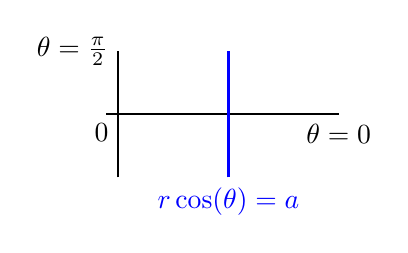
\begin{tikzpicture}[scale=0.4]
    %Axis
    \draw[thick] (-2.5ex,0) -- (7,0) node [below] {\(\theta=0\)};
    \draw[thick] (0,-2) 
    node [left] {} 
    -- (0,2) 
    node [left] {\(\theta=\frac{\pi}{2}\)};

    \node[anchor=north east] (Origin) at (0,0) {\(0\)};

    \draw[thick,blue] (3.5,-2) node [below] {\(r \cos(\theta)=a\)} -- (3.5,2);
  \end{tikzpicture}
\end{tabular} & \(x=a\)\\
\hline
\begin{tabular}{@{}Sc@{}}
  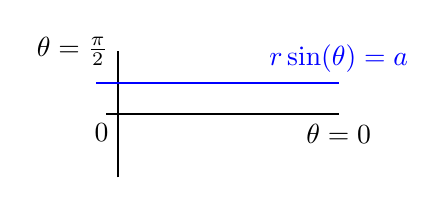
\begin{tikzpicture}[scale=0.4]
    %Axis
    \draw[thick] (-2.5ex,0) -- (7,0) node [below] {\(\theta=0\)};
    \draw[thick] (0,-2) 
    node [left] {} 
    -- (0,2) 
    node [left] {\(\theta=\frac{\pi}{2}\)};

    \node[anchor=north east] (Origin) at (0,0) {\(0\)};

    \draw[thick,blue] (-2em,1) -- (7,1) node [above] {\(r \sin(\theta)=a\)};
  \end{tikzpicture}
\end{tabular}& \(y=a\)\\
\hline
\begin{tabular}{@{}Sc@{}}
  \begin{tikzpicture}[scale=0.4]
    %Axis
    \draw[thick] (-2.5ex,0) -- (7,0) node [below] {\(\theta=0\)};
    \draw[thick] (0,-2) 
    node [left] {} 
    -- (0,2) 
    node [left] {\(\theta=\frac{\pi}{2}\)};

    \node[anchor=north east] (Origin) at (0,0) {\(0\)};

    \draw[thick,blue] (0,0) -- (7,2) node [above right] {\(\theta=\alpha\)};

    \coordinate (A) at (7,0);
    \coordinate (B) at (0,0);
    \coordinate (C) at (7,2);
    \pic[draw, -, blue, thick, "\small \(\alpha\) \normalsize", angle eccentricity=1.7] {angle = A--B--C};
  \end{tikzpicture}
\end{tabular}& \(y=x\tan(\alpha)\)\\
\hline
\begin{tabular}{@{}Sc@{}}
  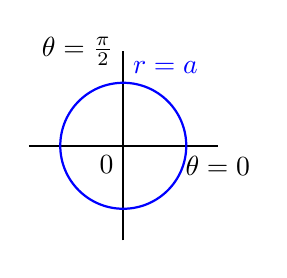
\begin{tikzpicture}[scale=0.4]
    %Axis
    \draw[thick] (-3,0) -- (3,0) node [below] {\(\theta=0\)};
    \draw[thick] (0,-3) 
    node [left] {} 
    -- (0,3) 
    node [left] {\(\theta=\frac{\pi}{2}\)};

    \node[anchor=north east] (Origin) at (0,0) {\(0\)};
    \node[above right, blue] (Circle) at (0,2) {\(r=a\)};
    \draw[thick,blue] (0,0) circle [radius=2cm];
  \end{tikzpicture}
\end{tabular}& \(x^2+y^2=a^2\)\\
\hline
\begin{tabular}{@{}Sc@{}}
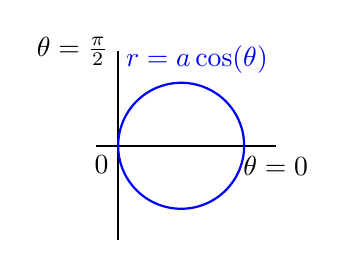
\begin{tikzpicture}[scale=0.4]
  %Axis
  \draw[thick] (-2em,0) -- (5,0) node [below] {\(\theta=0\)};
  \draw[thick] (0,-3) 
  node [left] {} 
  -- (0,3) 
  node [left] {\(\theta=\frac{\pi}{2}\)};

  \node[anchor=north east] (Origin) at (0,0) {\(0\)};
  \node[above, blue] (Circle) at (2.5,2) {\(r=a \cos(\theta)\)};
  \draw[thick,blue] (2,0) circle [radius=2cm];
\end{tikzpicture} 
\end{tabular}& \(\left(x-\frac{a}{2}\right)^2+y^2=\frac{a^2}{4}\)\\
\hline
\begin{tabular}{@{}Sc@{}}
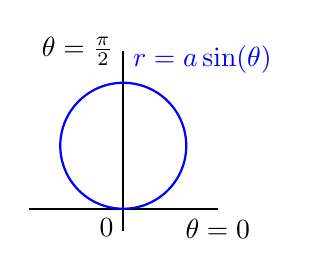
\begin{tikzpicture}[scale=0.4]
  %Axis
  \draw[thick] (-3,0) -- (3,0) node [below] {\(\theta=0\)};
  \draw[thick] (0,-2em) 
  node [left] {} 
  -- (0,5) 
  node [left] {\(\theta=\frac{\pi}{2}\)};

  \node[anchor=north east] (Origin) at (0,0) {\(0\)};
  \node[above right, blue] (Circle) at (0,4) {\(r=a \sin(\theta)\)};
  \draw[thick,blue] (0,2) circle [radius=2cm];
\end{tikzpicture} 
\end{tabular}& \(x^2+\left(y-\frac{a}{2}\right)^2=\frac{a^2}{4}\)\\
\hline
    \end{longtable}
    \item Tangent lines at the pole are obtained by solving \(r=0\).
    \item Know how to find range of \(r\) and \(\theta\) (given a func/eqn).
    \item \(r=f(\theta)\) is symmetrical about the polar (horizontal) axis iff \(f(\theta)=f(-\theta)\).
    \begin{itemize}
      \item Suppose \(r\) is a function of \(\cos(n\theta)\)\footnote{E.g.: \(r=a\sqrt{(4+\sin^2(\theta))^2\cos(\theta)}\)} \emph{only}. Then, the lines of symmetry are \(n\theta=0,\pi,2\pi,\ldots\)
    \end{itemize}
    \item \(r=f(\theta)\) is symmetrical about the vertical line \(\theta=\frac{\pi}{2}\) iff the equation \(f(\theta)=f(\pi-\theta)\).
    \begin{itemize}
      \item Suppose \(r\) is a function of \(\sin(n\theta)\) \emph{only}. Then, the lines of symmetry are \(n\theta=\frac{\pi}{2},\frac{3\pi}{2},\ldots,\frac{(2m+1)\pi}{2},\ldots\)
    \end{itemize}
    \item \(r=f(\theta)\) is symmetrical about the pole iff \((r,\theta)\) is a point on the curve whenever \((-r,\theta)\) is.
    \item \(R\)-formula may be necessary
    \item Area of a sector: \(A=\frac{1}{2}\int_{\alpha}^{\beta}r^2\,\text{d}\theta\), where \(\alpha<\beta\).
    \item Arc length\(=\int_{\theta_1}^{\theta_2} \sqrt{r^2+\left(\frac{dr}{d\theta}\right)^2}\,\text{d}\theta\)
  \end{itemize}
\end{stbox}
\begin{IN}
  \begin{enumerate}
    \item \(r\) is normally \(\geq 0\). But, in some questions, it can be negative.
    \item No need to fully expand; a final answer such as \((x^2+y^2)^2=3y(x^2+y^2)-4y^2\) suffices.
    \item Polar curve sketching essentials:
    \begin{enumerate}
      \item Shape of curve
      \item Intersection(s) with (`axial') half lines
      \item Nothing else \emph{unless} the qns asks for it
    \end{enumerate}
    \begin{enumerate}[label=\(\qed\)]
      \item Be careful of the sharpness / smoothness of points! Points supposed to be sharp should be sufficiently so, and those supposed to be smooth should be sufficiently rounded / not look sharp.
      \item Check whether the polar axes are tangents at pole. Use this information to draw accurate graphs.
      \item Best to add a small dotted line to show tangentiality at intercepts.
      \item Careful about constants like \(a\) in \(r=a\sin(\theta)\) for axial intercepts.
      \item No need to state points at the pole unless they are `axial', i.e. \(\theta=0\), or \(\frac{\pi}{2}\), etc.
    \end{enumerate}
    \item When finding maximum / minimum \(y\) values \(\left(\frac{dy}{d\theta}=0\right)\), we need to check its nature (1st/2nd deriv test). However, this is unnecessary for max / min \(r\) values.
    \item For stuff like \(\frac{dy}{dx}\), try to keep it in polar form if possible instead of converting to cartesian form.
    \item As usual, be \emph{careful}! E.g. Which values need to be rejected.
    \item When reflecting/rotating, a diagram may be useful in finding the necessary angle/expression to replace \(\theta\) with. E.g.: \small
    \begin{enumerate}
      \item In the case of reflecting about \(r=\theta\) or \(y=x\), \((r,\theta) \to (r,\frac{\pi}{2}-\theta)\).
      \item Reflect about the half-line \(\theta=\frac{\pi}{2}\) \(\implies\) \((r,\theta) \to (r,\pi-\theta)\).
    \end{enumerate} \normalsize
  \end{enumerate}
\end{IN}
\begin{lbox}[colbacktitle=white, coltitle=black, colframe=black]{G.C. Skills} 
  \begin{enumerate}
    \item Nice polar \(\implies\) Zoom fit + Zoom square
    \item Simply press alpha trace 1 to get \(r_1\). In fact, this works for the other modes available in the GC as well. 
    \item We can type \(\left. \frac{d}{d\theta}{r_1} \right\rvert_{\theta=\theta}\) info formulas (like the one for arc length) without having to manually differentiate it!
  \end{enumerate}
\end{lbox}

\chapter{Conic Sections}
\begin{definition}{}{}
  Eccentricity, \(e\), is defined as 
  \[\frac{\text{distance of \(P\) from focus}}{\text{distance of \(P\) from directrix}}.\]
\end{definition}
\begin{stbox}{General Information}{}
  \begin{itemize}[label=\(\circ\)]
    \item Shapes associated with the value of \(e\)
    \begin{itemize}
      \item \(e=0\): Circle
      \item \(0<e<1\): Ellipse 
      \item \(e=1\): Parabola
      \item \(e>1\): Hyperbola
    \end{itemize}
  \end{itemize}
  \resizebox{\columnwidth}{!}{\begin{tabular}{|Sc|Sc|Sc|Sc|Sc|Sc|Sc|}
    \hline 
    Conic & \multicolumn{2}{Sc|}{Parabolas} & \multicolumn{2}{Sc|}{Ellipses} & \multicolumn{2}{Sc|}{Hyperbolas}\\
    \hline
    Equation & \(x^2=4py\) & \(y^2=4px\) & 
    \(\begin{aligned}
      \frac{x^2}{a^2}+\frac{y^2}{b^2}=1\text{, }a>b
    \end{aligned}\) & 
    \(\begin{aligned}
    \frac{x^2}{a^2}+\frac{y^2}{b^2}=1\text{, }b>a
    \end{aligned}\) &
    \(\begin{aligned}
    \frac{x^2}{a^2}-\frac{y^2}{b^2}
    \end{aligned}\) & 
    \(\begin{aligned}
    \frac{y^2}{b^2}-\frac{x^2}{a^2}=1
    \end{aligned}\)\\
    \hline
    Foci & \((0,p)\) & \((p,0)\) & \((\pm c,0)\) & \((0,\pm c)\) & \((\pm c,0)\) & \((0,\pm c)\)\\
    \hline
    \(a,b,c\) & \multicolumn{2}{Sc|}{N.A.} & \(c^2=a^2-b^2\) & \(c^2=b^2-a^2\) & \multicolumn{2}{Sc|}{\(c^2=a^2+b^2\)}\\
    \hline
    Directrices & \(y=-p\) & \(x=-p\) & 
    \(\begin{aligned}
      x=\pm\frac{a}{e}=\pm\frac{a^2}{c}
    \end{aligned}\) & 
    \(\begin{aligned}
    y=\pm\frac{b}{e}=\pm\frac{b^2}{c}
    \end{aligned}\) & 
    \(\begin{aligned}
    x=\pm\frac{a}{e}=\pm\frac{a^2}{c}\end{aligned}\) & 
    \(\begin{aligned}
    y=\pm\frac{b}{e}=\pm\frac{b^2}{c}
    \end{aligned}\)\\
    \hline
    \multirow{2}{*}{e} & \multicolumn{2}{Sc|}{\(e=1\)} & \multicolumn{2}{Sc|}{\(0<e<1\)} & \multicolumn{2}{Sc|}{\(e>1\)}\\
    \cline{2-7}
    & \multicolumn{2}{Sc|}{N.A.} & 
    \(\begin{aligned}
      e&=\frac{c}{a}\\
      &=\frac{\sqrt{a^2-b^2}}{a}\\
      &=\sqrt{1-\frac{b^2}{a^2}}
    \end{aligned}\) & 
    \(\begin{aligned}
      e&=\frac{c}{b}\\
      &=\frac{\sqrt{b^2-a^2}}{b}\\
      &=\sqrt{1-\frac{a^2}{b^2}}
    \end{aligned}\) & 
    \(\begin{aligned}
      e&=\frac{c}{a}\\
      &=\frac{\sqrt{a^2+b^2}}{a}\\
      &=\sqrt{1+\frac{b^2}{a^2}}
    \end{aligned}\) & 
    \(\begin{aligned}
      e&=\frac{c}{b}\\
      &=\frac{\sqrt{a^2+b^2}}{b}\\
      &=\sqrt{1+\frac{a^2}{b^2}}
    \end{aligned}\)
    \\
    \hline
    \begin{tabular}{@{}Sc@{}}
      Reflective\\
      Property
    \end{tabular} &
    \multicolumn{2}{p{3cm}|}{
      \begin{minipage}{3cm}
        \vspace{1mm}\small When light parallel to its axis of symmetry (\(x=0\) or \(y=0\)) hits its concave side, the light is reflected to the focus.\\[1mm]
    \end{minipage}}  &
    \multicolumn{2}{p{5.5cm}|}{ 
    \begin{minipage}{5.5cm}
      \small For any point \(P\) on the ellipse with\\ \(a>b\),
      \[PF_1+PF_2=2a\]
    \end{minipage}}
     & \multicolumn{2}{p{5cm}|}{
    \begin{minipage}{5cm}
      \small For any point \(P\) on the hyperbola with \(\operatorname{coeff}(x^2)>0\),
      \[\lvert PF_1-PF_2 \rvert=2a\]
    \end{minipage}}\\
    \hline
  \end{tabular}}
  \newpage
  \begin{itemize}[label=\(\circ\)]
    \item Polar Form: \(x=p\), \(x=-p\), \(y=p\), or \(y=-p\) being the directrix
  \end{itemize}
  \begin{center}
    \begin{tabular}{p{3cm}p{3cm}p{3cm}}
      & \begin{tabular}{|p{3cm}|}
        \hline
        \centering Top\\
        \[r=\frac{ep}{1+e\sin(\theta)}\]
      \end{tabular} &\\
      \begin{tabular}{|p{3cm}}
        \hline
        \centering Left\\
        \[r=\frac{ep}{1-e\cos(\theta)}\]
      \end{tabular} &
      \begin{tabular}{|p{3cm}|}
        \hline
        \centering \vphantom{Top}\\
        \[\vphantom{r=\frac{ep}{1+e\sin(\theta)}}\]
      \end{tabular} & 
      \begin{tabular}{p{3cm}|}
        \hline
        \centering Right\\
        \[r=\frac{ep}{1+e\cos(\theta)}\]
      \end{tabular}\\
      \begin{tabular}{p{3cm}}
        \hline
        \centering \vphantom{Top}\\
        \[\vphantom{r=\frac{ep}{1+e\sin(\theta)}}\]
      \end{tabular} &
      \begin{tabular}{|p{3cm}|}
        \hline
        \centering Bottom\\
        \[r=\frac{ep}{1-e\sin(\theta)}\]
      \end{tabular}
      & 
      \begin{tabular}{p{3cm}}
        \hline
        \centering \vphantom{Top}\\
        \[\vphantom{r=\frac{ep}{1+e\sin(\theta)}}\]
      \end{tabular}\\
      & \begin{tabular}{p{3cm}}
        \hline \hphantom{1}   
      \end{tabular} &
    \end{tabular}
  \end{center}
\end{stbox}
  \begin{definition*}{}{}
    \begin{itemize}[label=\(\circ\)]
      \item Major / minor axes \(\implies\) lengths of longest and shortest diameters respectively.
      \item Semi-major / semi-minor \(\implies\) half of major / minor axes respectively.
      \item Focal radius \(\implies\) distance from point on conic section to focus.
    \end{itemize}
  \end{definition*}
  \begin{note}
    Some possible things to try:
    \begin{itemize}
      \item Using the fact that \(PF_1+PF_2=2a\) to do simultaneous equations.
      \item Converting to polar form (when \(e<1\) so \(r \geq 0\)) for distances.
      \item Congruent/Similar triangles.
      \item Classic use of discriminants.
      \item Sum and product of roots: Given any polynomial \(ax^2+bx+c\) with the roots \(\alpha\) and \(\beta\),
      \[\alpha + \beta = - \frac{b}{a} \qquad\text{and}\qquad \alpha\beta=\frac{c}{a}.\]
    \end{itemize}
  \end{note}
\chapter{Functions}
\begin{stbox}{General Information}
  \begin{enumerate}
    \item Horizontal Line Test: 
    \begin{enumerate}
      \item Fail: Since\footnote{some specific \(k\), e.g. \(y=1/2\)} \(y=k\) intersects the graph of \(y=f(x)\) more than once, therefore \(f\) is not injective.
      \item Success: Since \emph{any} horizontal line \(y=k\) will intersect the graph of \(y=g(x)\) \emph{at most once}, so \(f(x)\) is one-one.
    \end{enumerate}  
    \item The inverse function, \(f^{-1}\), of a function \(f\) exists iff \(f\) is one-one.
    \item \(y=f^{-1}\) is a reflection of \(y=f(x)\) about the line \(y=x\).
    \item The composite function \(gf\) exists iff \(R_f \subseteq D_g\).
    \item \(D_{gf}=D_f\) \& \(R_{gf}=R_g\).
    \item Finding the range:
    \begin{enumerate}
      \item Graphing method:
      \item Mapping method, e.g.: \(\begin{tikzcd}
        {D_f=(0, \infty)} & {(1,\infty)} & {(0,\infty)=R_{gf}} & {} & {}
        \arrow["f", from=1-1, to=1-2]
        \arrow["g", from=1-2, to=1-3]
      \end{tikzcd}\)
    \end{enumerate} 
  \end{enumerate}
\end{stbox}

\chapter{Permutations and Combinations}
\begin{definition}{}{}
  The terms \(n\) \emph{pick} \(r\) and \(n\) \emph{choose} \(r\) respectively denote 
  \[{^n}P_r := \frac{n!}{(n-r)!} \qquad\text{and}\qquad \binom{n}{r}={^n}C_r:=\frac{n!}{(n-r)!r!}.\]
\end{definition}
\begin{stbox}{General Information}
  \begin{itemize}
    \item Addition and multiplication principles
    \item Know how to `bundle' objects together so as to calculate the total no. of permutations.
    \item There are \(\frac{n!}{n_1!n_2!\cdots n_r!}\) number of ways to arrange \(n\) objects, of which \(n_1\) are `similar', \(n_2\) are `alike', \ldots, \(n_r\) are `the same'.
  \end{itemize}
\end{stbox}
    \begin{fact}
      Intuition: If there are \(n_1\) objects are non-distinct out of \(n\) objects, then there are \(n_1!\) ways to arrange these objects that results in `the same' permutation.
    \end{fact}
  \begin{stbox}{}
  \begin{itemize}
    \item Case-wise considerations/calculations (then summing together the total number of permutations)
    \item Unordered circular permutations:\\
    There are \(\frac{n!}{n}=(n-1)!\) number of ways of arranging \(n\) distinct objects in a circle.
  \end{itemize}
\end{stbox}
    \begin{fact}
      For unordered circular permutations, we do not care if you rotate the seating arrangement, as long as neighbours are preserved for each object. i.e. \((A,B,C,D) \sim (B,C,D,A)\). As a result, each such collection of \(n\) permutations reduces down to one. Thus, explaining the division by \(n\).
    \end{fact}
\begin{stbox}{}
\begin{itemize}
    \item Complementary Method, i.e. taking number of arrangements without restriction - number of arrangements with the opposite of that restriction.
\end{itemize}
\end{stbox}
    \begin{example}{}{}
      Number of ways two girls \emph{cannot} sit next to each other = number of arrangements \emph{without restriction} \(-\) number of arrangements with girls sitting \emph{together}.
    \end{example}
\begin{stbox}{}
\begin{itemize}
    \item Insertion Method, place down some of your objects and then insert the rest in the gaps.
  \end{itemize}
\end{stbox}
    \begin{example}{}{}
      \begin{enumerate}[label={}]
        \item Boys sit at table first: \(2!\) ways.
        \item \vspace{-1mm} From the 3 gaps, choose 2 for the 2 girls to sit at: 3 ways.
        \item \vspace{-1mm} The girls can arrange themselves in \(2!\) ways.
        \item \vspace{-1mm} So, total no. of ways is \(2! \cdot 3 \cdot 2!=12\).
      \end{enumerate}
    \end{example}
\begin{stbox}{}
\begin{itemize}
    \item Ordered circular permutations: First calculate the number of unordered permutations, then add the ordering at the end.
  \end{itemize}
\end{stbox}
    \begin{note}
      Circular arrangements are not the same as row arrangements.
      
      We know that \(A\) and \(B\) are not considered to be seating together in the row arrangement of \((A,C,D,E,B)\). But, they are seating together in a corresponding row arrangement. The number of row arrangements can be less than, equal to, or more than the number of circular arrangements.
    \end{note}
\chapter{Vectors}
\begin{longtable}{|Sc|Sc|}
  \hline
  Lines & Planes\\
  \hline
  \multicolumn{2}{|Sc|}{Equivalent Forms}\\
  \hline
  \begin{minipage}{0.5\textwidth}
    \begin{enumerate}
      \item Vector Equation: \[\ell \colon \mathbf{r}=\mathbf{a}+\lambda \mathbf{m}\text{, }\lambda \in \mathbb{R},\]
      \item Cartesian Equation: 
      \[\frac{x-a_1}{m}=\frac{y-a_2}{m_2}=\frac{z-a_3}{m_3.}\]
    \end{enumerate}
\end{minipage} & 
\begin{minipage}{0.5\textwidth}
\begin{enumerate}
  \item Vector Equation: 
  \[\Pi \colon \mathbf{r}=\mathbf{a}+\lambda
  \mathbf{m_1}+\mu \mathbf{m_2}\text{ where }\lambda,\mu\in\mathbf{R},\]
  \item Scalar Product Form: 
  \[\Pi \colon \mathbf{r} \cdot \mathbf{n}=p\]
  where the scalar \(p:= \mathbf{a}\cdot \mathbf{n}\),
  \item Cartesian Equation:
  \[n_1x+n_2x+n_3z=p\]
  where the normal vector\\
  \(\mathbf{n}:=\begin{pmatrix}
    n_1 & n_2 & n_3
  \end{pmatrix}^\top\).
\end{enumerate}
\end{minipage}\\
\hline
\multicolumn{2}{|Sc|}{Foot of Perpendicular}\\
\hline
\begin{minipage}{0.5\textwidth}
  \begin{enumerate}
    \item[M1:] 
    \begin{enumerate}
      \item \(\overrightarrow{ON}=\mathbf{a}+\lambda \mathbf{m}\),
      \item \(\overrightarrow{QN} \cdot \mathbf{m}=0\), solve for \(\lambda\),
      \item Substitute \(\lambda\) into (a).
    \end{enumerate}
    \item[M2:] 
    \begin{enumerate}
      \item \(\overrightarrow{AN}=\left(\overrightarrow{AQ} \cdot \mathbf{\hat{m}}\right)\mathbf{\hat{m}}\),
      \item \(\overrightarrow{ON}=\overrightarrow{OA}+\overrightarrow{AN}\).
    \end{enumerate}
  \end{enumerate}
\end{minipage} & 
\begin{minipage}{0.5\textwidth}
  \begin{enumerate}[label=(\alph*)]
    \item \(\ell_{NQ} \colon \mathbf{r}=\overrightarrow{OQ}+\lambda n\), where \(\lambda \in \mathbb{R}\), and \(\Pi \colon \mathbf{r}\cdot \mathbf{n}= \mathbf{a}\cdot \mathbf{n}\),
    \item \(\left(\overrightarrow{OQ}+\lambda \mathbf{n}\right)\cdot \mathbf{n}= \mathbf{a}\cdot \mathbf{n}\), solve for \(\lambda\),
    \item \(\overrightarrow{ON}+\overrightarrow{OQ}+\lambda \mathbf{n}\).
  \end{enumerate}
\end{minipage}\\
\hline
\multicolumn{2}{|Sc|}{Shortest Distance of Point To Line, \(QN\)}\\
\hline
\begin{minipage}{0.5\textwidth}
  \begin{enumerate}
    \item[M1:] \(\norm{\overrightarrow{AQ} \times \mathbf{\hat{m}}}\).
    \item[M2:]
    \begin{enumerate}
      \item \(AN= \norm{\overrightarrow{AQ}\cdot \mathbf{\hat{m}}} \),
      \item Pythagoras' Theorem.
    \end{enumerate}
    \item[M3:] Using the foot of perpendicular, find distance \(QN\).
  \end{enumerate}
\end{minipage} &
\begin{minipage}{0.5\textwidth}
  \begin{enumerate}
    \item[M1:] \(\norm{\overrightarrow{AQ}\cdot \mathbf{\hat{n}}} \).
    \item[M2:] for distance of plane to \emph{origin}: If \(\Pi \colon \mathbf{r}\cdot \mathbf{n}=p\), \(\frac{p}{\norm{\mathbf{n}}}\) is the shortest distance from the origin to the plane \(\Pi\). \emph{Note:}
    \begin{itemize}
      \item If \(\frac{p}{\norm{\mathbf{n}}}>0\), then \(\Pi\) `above' \(0\).
      \item If \(\frac{p}{\norm{\mathbf{n}}}<0\), then \(\Pi\) `below' 0.
    \end{itemize}
    \item[M3:] Using the foot of perpendicular, then find distance \(QN\).
  \end{enumerate}
\end{minipage}\\
\hline
\newpage
\hline
Relationship Btw 2 Lines & Relationship Btw Line \& Plane\\
\hline
\begin{minipage}{0.5\textwidth}
  \begin{enumerate}
    \item Parallel, Non-Intersecting
    \begin{enumerate}
      \item \(\mathbf{m_1}\newparallel \mathbf{m_2}\),
      \item Solving \(\ell_1=\ell_2\) gives no real solution.
    \end{enumerate}
    \item Parallel, Coinciding
    \begin{enumerate}
      \item \(\mathbf{m_1}\newparallel \mathbf{m_2}\),
      \item \(\mathbf{a}\) lies in \(\ell_1\) and \(\ell_2\).
    \end{enumerate}
    \item Non-Parallel, Intersecting
    \begin{enumerate}
      \item \(\mathbf{m_1}\) not \(\newparallel \mathbf{m_2}\),
      \item Solve \(\ell_1=\ell_2\) to find intersection.
    \end{enumerate} 
    \item Skew Lines\\
    (Non-Parallel, Non-Intersecting)
    \begin{enumerate}
      \item \(\mathbf{m_1}\) not \(\newparallel \mathbf{m_2}\),
      \item Solving \(\ell_1=\ell_2\) gives no real solution. 
    \end{enumerate}
  \end{enumerate}
\end{minipage} &
\begin{minipage}{0.5\textwidth}
  \begin{enumerate}
    \item \(\ell\) lies in \(\Pi\)
    \begin{enumerate}[label=M\arabic*:]
      \item
      \begin{enumerate}
        \item \(\mathbf{m}\cdot \mathbf{n}=0\) says \(\ell \newparallel \Pi\),
        \item Combined with \(\mathbf{a}\cdot \mathbf{n}=p\), we conclude \(\ell\) lies in \(\Pi\).
      \end{enumerate}
      \item Substitute \(\ell\) into \(\Pi\) and show the system (of lin eqns) is consistent for all \(\lambda\).
    \end{enumerate}
    \item \(\ell \newparallel \Pi\) but Nonintersecting
    \begin{enumerate}[label=M\arabic*:]
      \item 
      \begin{enumerate}
        \item Show \(\mathbf{m}\cdot \mathbf{n}=0\), so \(\ell \newparallel \Pi\).
        \item Then \(\mathbf{a}\cdot \mathbf{n} \neq p\), tells us \(\ell\) and \(\Pi\) are nonintersecting.
      \end{enumerate}
      \item Substitute \(\ell\) into \(\Pi\), and show the system (of lin eqns) is inconsistent.
    \end{enumerate} 
    \item Intersect at 1 point
    \begin{enumerate}[label=M\arabic*:]
      \item \(\mathbf{m}\cdot \mathbf{n} \neq 0\).
    \end{enumerate}
    To find point of intersection:
    For the plane \(\Pi\) and \(\ell\) defined by
    \(\begin{aligned}
      \Pi &\colon \mathbf{r}\cdot \mathbf{n}=p\\
      \ell &\colon \mathbf{r}=\mathbf{a}+\lambda \mathbf{m}
    \end{aligned}\)
    Solve for \(\lambda\) using simultaneous equations or G.C.
  \end{enumerate}
\end{minipage}\\
\hline
- & Relationship Btw 2 Planes\\
\hline &
\begin{minipage}{0.5\textwidth}
  \begin{enumerate}
    \item Parallel Planes: Show there exists an \(\mathbf{a}\) for which
    \begin{enumerate}
      \item \(\mathbf{a}\cdot \mathbf{n_1}= p_1\),
      \item \(\mathbf{a}\cdot \mathbf{n_2}\neq p_2\).
    \end{enumerate}
    \item Same Plane: Show there exists an \(\mathbf{a}\) for which
    \begin{enumerate}
      \item \(\mathbf{a}\cdot \mathbf{n_1}= p_1\),
      \item \(\mathbf{a}\cdot \mathbf{n_2}= p_2\).
    \end{enumerate}
    \item Intersect in a line \(\ell\); To find this line:
    \begin{enumerate}[label=M\arabic*:]
      \item \(\mathbf{n_1}\times \mathbf{n_2}\) gives the direction vector. So find a common point with simultaneous equations.
      \item Solving system of linear equations, from the \emph{cartesian} form of the planes, using G.C.
    \end{enumerate}
  \end{enumerate}
\end{minipage}\\
\hline
\multicolumn{2}{|Sc|}{Point of Reflection}\\
\hline
\multicolumn{2}{|Sc|}{  
\begin{minipage}{\textwidth}
\begin{center}
  \begin{enumerate*}[itemjoin={,\qquad\qquad}]
    \item Find foot of perpendicular \(\overrightarrow{ON}\)
    \item Notice \(\overrightarrow{OA'}=\overrightarrow{OA}+2\overrightarrow{AN}=2\overrightarrow{ON}-\overrightarrow{OA}\).
  \end{enumerate*}
\end{center}
\end{minipage}}\\
  \hline
  \multicolumn{2}{|Sc|}{
    \begin{tabular}{Sc|Sc|Sc}
      \multicolumn{3}{Sc}{Angle Between}
    \end{tabular}}\\
      \hline
  \multicolumn{2}{|Sc|}{
    \begin{tabular}{Sc|Sc|Sc}
      \begin{minipage}{0.333\textwidth}
        2 Lines
      \end{minipage} &
      \begin{minipage}{0.333\textwidth}
        Line and Plane
      \end{minipage} &
      \begin{minipage}{0.333\textwidth}
        2 Planes
      \end{minipage}
    \end{tabular}}\\
    \hline
  \multicolumn{2}{|Sc|}{
    \begin{tabular}{Sc|Sc|Sc}
      \begin{minipage}{0.333\textwidth}
        \[\theta=\cos^{-1}\left\lvert \mathbf{\widehat{m}_1}\cdot {\mathbf{\widehat{m}_2}}\right\rvert.\]
      \end{minipage} &
      \begin{minipage}{0.333\textwidth} 
        \[\theta=\sin^{-1}\left\lvert \mathbf{\widehat{m}}\cdot \mathbf{\widehat{n}} \right\rvert .\]
      \end{minipage} &
      \begin{minipage}{0.333\textwidth}
        \[\theta=\cos^{-1}\left\lvert \mathbf{\widehat{n}_1}\cdot \mathbf{\widehat{n}_2} \right\rvert.\]
      \end{minipage}\\
    \end{tabular}
  }\\
  \hline
\end{longtable}
\chapter{Probability}
\begin{stbox}{General Information}
  \begin{enumerate}
    \item Principle of Inclusion and Exclusion for
    \begin{enumerate}
      \item Two events:
      \[\Prob(A \cup B)=\Prob(A)+\Prob(B)-\Prob(A \cap B),\]
      \item Three events:
      \[\Prob(A \cup B \cup C)=\Prob(A)+\Prob(B)+\Prob(C)-\Prob(A\cap B)-\Prob(A \cap C)-\Prob(B \cap C)+\Prob(A \cap B \cap C).\]
    \end{enumerate}
    \item Mutually Exclusive Events:
    \begin{align*}
      \Prob(A \cap B)&=0,\\
      \Prob(A \cup B)&=\Prob(A)+\Prob(B).
    \end{align*}
    \item Independent Events:
    \begin{align*}
      \Prob(A \,\vert\, B)&=\Prob(A),\\
      \Prob(A \cap B)&=\Prob(A)\Prob(B).
    \end{align*}
    \item Conditional Probability:
    \[\Prob(A \,\vert\, B)=\frac{\Prob(A \cap B)}{\Prob(B)}.\]
    \item Use PnC to help compute stuff faster.
    \item When we want to find the greatest and least possible probability (e.g. of \(\Prob(A^\complement\cap B^\complement\cap C^\complement)\)), it is advisable to draw a Venn diagram and fill in all relevant probabilities. 
  \end{enumerate}
\end{stbox}
\begin{example}{}{}
  There are 6 white balls and 5 black balls. Two are randomly drawn. What is the probability that one is white and the other black?
  \begin{align*}
    \left(\frac{5}{11}\right)\left(\frac{6}{10}\right)+\left(\frac{6}{11}\right)\left(\frac{5}{10}\right)=\frac{6}{11} \qquad&\text{vs}\qquad \frac{\binom{6}{1}\binom{5}{1}}{\binom{11}{2}}=\frac{6}{11}.
  \end{align*}
\end{example}

\chapter{Differential Equations}
\section{First Order D.E.s}
\subsection{Elementary Solving Techniques}
\begin{stbox}{General Information}
  \begin{enumerate}
    \item Separable Variables:
    \begin{align*}
      \frac{dy}{dx}&=f(y)g(x),
      \int \frac{1}{f(y)}\,dy=\int g(x)\,dx.
    \end{align*}
    \item Integrating Factor:
    \begin{align*}
      \frac{dy}{dx}+P(x)y&=Q(x),\quad\text{let I.F.}=e^{\int P(x)\,dx}\\
      e^{\int P(x)\,dx} \frac{dy}{dx}+ye^{\int P(x)\,dx}P(x)&=Q(x)e^{\int P(x)\,dx},\\
      ye^{\int P(x)\,dx}&=\int Q(x)e^{\int P(x)\,dx}\,dx.
    \end{align*}
  \end{enumerate}
\end{stbox}
\subsection{Numerical Methods}
\begin{stbox}{General Information}
  \begin{enumerate}
    \item Euler's Method: 
    \[y_{i+1}+hf(x_i,y_i).\]
  \end{enumerate}
\end{stbox}
    \begin{example}{}{}
      Let (step size) \(h=0.25\) and \(f(x,y)=\frac{dy}{dx}\):
      \begin{align*}
        \text{By MF26,}\quad y_2&=\frac{2}{3}+hf\left(0,\frac{2}{3}\right)\\
        &=\frac{13}{18}\\[3mm]
        y_3&=\frac{13}{18}+hf\left(0.25,\frac{13}{18}\right)\\
        &=0.6701865657.\\[3mm]
        \text{Therefore, }y(0.5)&\approx 0.670.
      \end{align*}
    \end{example}
    \begin{stbox}{}
      \setcounter{enumi}{1}
    \begin{enumerate}
    \item Improved Euler's Method: 
    \[i_{i+1}=y_i+hf(x_i,y_i)\quad\&\quad y_{i+1}=y_i+\frac{h}{2}[f(x_i,y_i)+f(x_{i+1},u_{i+1})].\]
    \item Error:
    \begin{enumerate}
      \item If \(\frac{dy}{dx}\) can be shown to be \emph{increasing} from the calculations of \(f(x,y)\), then the curve is \emph{concave upwards}, leading to a \emph{underestimate}.
      \item If \(\frac{dy}{dx}\) can be shown to be \emph{decreasing} from the calculations of \(f(x,y)\), then the curve is \emph{concave downwards}, leading to a \emph{overestimate}.
    \end{enumerate}
  \end{enumerate}
\end{stbox} ~
\begin{example}{}{}
  From the computation, \emph{the values of} \(\frac{dy}{dx}\) \emph{increases}, i.e. \(\frac{d^2y}{dx^2}>0\), and thus implying the solution curve to be \emph{concave upwards}. Therefore, we have an \emph{underestimation}. 
\end{example}
\begin{example}{Misc}{}
  It is suggested that the estimation in part (ii)\footnote{Given the point (1,1), we estimated the value of y(2) using the Improved Euler's Method} can be further improved by reducing the step size. Sketch the solution curve and hence comment on this suggestion.\\[3mm]
  The solution curve has a \emph{stationary point at} \(x=1.47\), which is between 1 and 2 and also the gradient of the curve is close to zero for \(x\) value beyond this stationary point. Thus, when the step size is reduced, \emph{tangent} at point close to this stationary point becomes \emph{almost parallel} to the curve, making \emph{little improvement} to the estimation due to \emph{little difference in} \(y\). 
\end{example}
\begin{example}{}{}
  It is found that the approximation obtained in (i) for the \(y\)-coordinate where \(x=0.75\) is an underestimation and has a percentage error of 120.633\%. Explain why there is such a substantial error.\\[3mm]
  From gradient values calculated above, we suspect sharp charges in gradient values within the interval (from negative to positive). Yet \emph{Euler's Method\footnote{We are explaining what it does} simply uses a straight line segment} with gradient\footnote{Emphasising negative gradient (Show its value)} \(-4.6409\) to estimate the curve for the first iteration, which could have lead to a significant underestimation of the \(y\)-value.
\end{example}
\begin{example}{}{}
  Compare the relative merits of Euler's Method and the Improved Euler's Method.
  \begin{enumerate}[wide=0pt, leftmargin=*]
    \item[Euler's Method:] It is computationally simpler.
    \item[Improved Euler's Method] More accurate as it takes the mean of the initial and next gradient. 
  \end{enumerate}
\end{example}
\section{Second Order D.E.}
\begin{center}
  \begin{tabular}{|Sc|Sc|}
    \hline
    \multicolumn{2}{|Sc|}{\textbf{Homogenous}}\\
    \hline
    Roots & Solution \(y_c\)\\
    \hline
    \(m_1 \neq m_2\) & \(y=Ae^{m_1x}+Be^{m_2x}\)\\
    \hline
    \(m:=m_1=m_2\) & \(y=(Ax+B)e^{mx}\)\\
    \hline
    \(m=\highlight[red!30]{p} \pm qi\) & \(y=e^{\highlight[red!30]{p}x}(A \cos(qx)+B \sin(qx))\)\\
    \hline
    \multicolumn{2}{|Sc|}{\textbf{Non-Homogenous, }\(c_2 \frac{d^2y}{dx^2}+c_1 \frac{dy}{dx}+c_0y=f(x)\)}\\
    \hline
    \multicolumn{2}{|Sc|}{\(y=y_c+y_p\) (C.F. + P.I.)}\\
    \hline
    \(f(x)\) & Trial Function for P.I.\\
    \hline
    Degree \(n\) polynomial & \(y_p=\sum_{i=0}^{n}a_ix^i\)\\
    \hline
    \(ke^{ax}\) & \(y_p=ae^{ax}\).\\
    \hline
    \(\alpha \cos(kx) +\beta \sin(kx)\) & \(y_p=a\cos(kx)+b\sin(kx)\)\\
    \hline
  \end{tabular}
  \begin{note}
    If \(y_c\) and \(f(x)\) share some common term, then \(y_p\) should be multiplied by \(x\) (some least \(i \in \mathbb{N}\) times till \(x^iy_p\) has no common term with \(y_c\)).  
  \end{note}
  \begin{example}{}{}
    \begin{enumerate}
      \item If \(y_c=A^{-3x}\) and \(f(x)=10e^x\), then \(y_p=kxe^x\)
      \item If \(y_c=Ae^x+Be^{-3x}\) and \(f(x)=10e^x\), then \(y_p=kxe^x\).
      \item If \(y_c=Ae^x+Bxe^{x}+Ce^{-3x}\) and \(f(x)=10e^x\), then \(y_p=kx^2e^x\).
    \end{enumerate}
  \end{example}
\end{center}
\section{Applications}
\subsection{Exponential Growth}
\begin{stbox}{General Information}
  Let \(k\) be the \emph{per-capita growth rate}\footnote{i.e. after accounting for births and deaths.} and \(P(t)\) be the population at time \(t\). Then we have the model:
  \[\frac{dP}{dt}=kP,\]
  with the solution
  \[P(t)=P_0e^{kt}.\]
\end{stbox}
\subsection{Logistics Growth}
\begin{stbox}{General Information}
  Let \(k\) be the \emph{per-capita growth rate}\footnote{i.e. after accounting for births and deaths.}, \(P(t)\) be the population at time \(t\), and \(N\) be the \emph{carrying capacity} of the system. Then we have the model:
  \[\frac{dP}{dt}=kP\left(1-\frac{P}{N}\right).\]
  \begin{enumerate}
    \item Without solving the logistics equation, we can sketch the solution curve by noting the sign of \(\frac{dP}{dt}\):
    \begin{enumerate}
      \item Equilibrium population values occur at \(P=0\) and \(P=N\).
      \item If, for instance \(k>0\),
      \begin{enumerate}[wide=0pt, leftmargin=*]
        \item[\(0<p<N\):] \(1-\frac{P}{N}>0\) so \(\frac{dP}{dt}>0\),
        \item[\(P>N\):] \(1-\frac{P}{N}<0\) so \(\frac{dP}{dt}<0\).  
      \end{enumerate}
    \end{enumerate}
    ``As \(t\) increases,  the population of \rule{1cm}{0.1mm}  increases to the stable population of \rule{1cm}{0.1mm}.''
  \end{enumerate}
\end{stbox}
\begin{example}{Neat trick of letting \(A=\pm \text{constant}\)}{}
  \begin{align*}
    \frac{dP}{dt}&=3P\left(1-\frac{P}{200}\right),\\
    \int \frac{1}{3P}+\frac{1}{600-3P}\,dP &= \int 1 \,dt,\\
    \ln \abs{\frac{3P}{600-3P}}&=3t+3c,\\
    \frac{3P}{600-3P}&=Ae^{3t}\text{, where }\highlight[red!30]{A=\pm e^{3c}},\\
    P&=\frac{200A}{A+e^{-3t}}
  \end{align*}
\end{example}
\begin{center}
  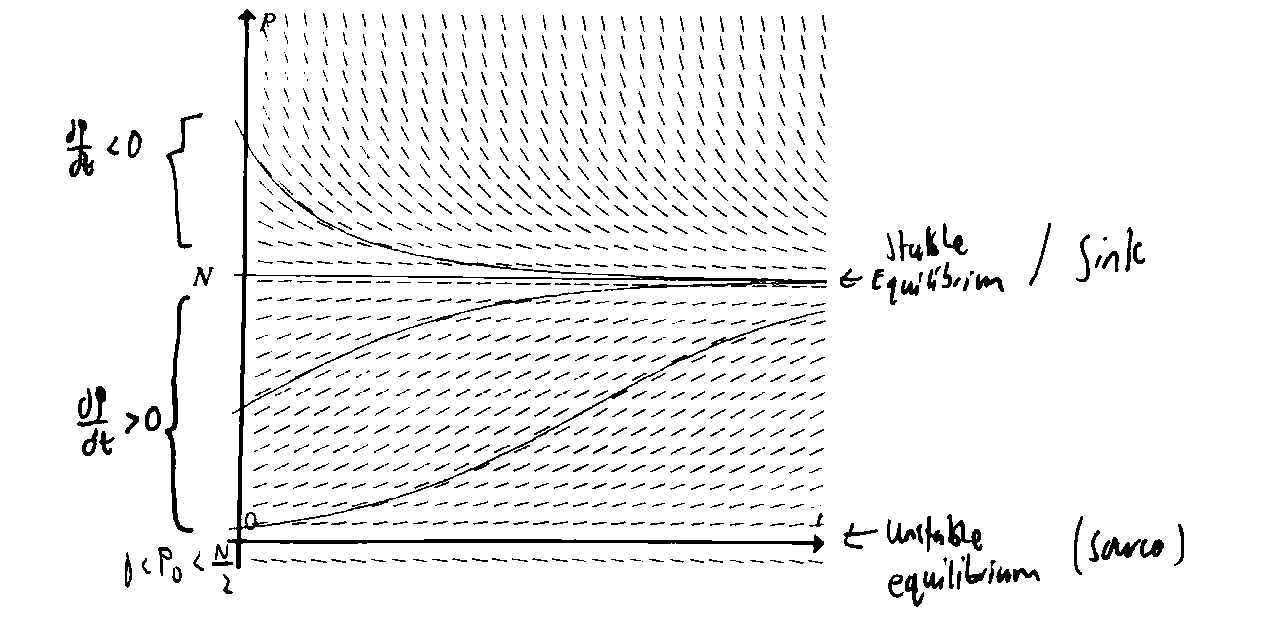
\includegraphics[width=\textwidth]{Logistics Curve}
\captionof{figure}{Logistics curve}
\end{center}
\newpage
\subsection{Harvesting}
\begin{stbox}{General Information}
  Let \(k\) be the \emph{per-capita growth rate}, \(P(t)\) be the population at time \(t\), \(N\) be the \emph{carrying capacity} of the system, and \(H\) the constant \emph{harvesting rate}. Then we have the model:
  \[\frac{dP}{dt}=kP\left(1-\frac{P}{N}\right)-H.\]
\begin{enumerate}
  \item Bifurcation Point
  \begin{enumerate}
    \item When \(0 \leq H<\frac{kN}{4}\), there are two equilibrium points, \(P=\frac{N}{2}\pm \sqrt{\frac{N^2}{4}-\frac{HN}{k}}\).
    \item When \(H=\frac{kN}{4}\), there is one equilibrium point at \(P=\frac{N}{2}\) (the bifurcation point).
    \item When \(H>\frac{kN}{4}\), there is no equilibrium point
  \end{enumerate}
  \item For Non-Extinction: 
  \begin{align*}
    \quad\frac{N^2}{4}-\frac{HN}{k} \geq 0 \qquad\text{and}\qquad P_0 \geq 450-\sqrt{\frac{N^2}{4}-\frac{HN}{k}}.
  \end{align*}
\end{enumerate}
\end{stbox}

\subsection{Physics}
\begin{stbox}{General Information}
  \textbf{MUST} rmb the forms.
  \begin{enumerate}
    \item Spring System (where \(k>0\) is the spring constant) 
    \[\ddot{x}+\frac{k}{m}x=0.\]
    Solution: use \(\highlight[red!30]{\text{R-formula}}\) to convert to \(A \cos(\omega t + \phi)\) where angular frequency \(\omega=\sqrt{\frac{k}{m}}\). Period \(T=\frac{2\pi}{\omega}=2\pi \sqrt{\frac{m}{k}}\).
    \item Simple Pendulum (where \(\ell\) is its length)
    \[\ddot{x}+\frac{g}{\ell}x=0.\]
    Angular frequency \(\omega=\sqrt{\frac{g}{\ell}}\) and period \(T=2\pi \sqrt{\frac{\ell}{g}}\).
    \item Spring-Mass-Dashpot System (where \(c>0\) is the damping constant)
    \[\ddot{x}+\frac{c}{m}\dot{x}+\frac{k}{m}x=0.\]
    Solution
    \begin{enumerate}
      \item Real and Distinct Roots: \emph{Overdamped}
      \item Identical Real Roots: \emph{Critically Damped}
      \item Complex Conjugate Roots: \emph{Underdamped}\\
      \emph{``It will oscillate about the equilibrium position with decreasing amplitude.''}
    \end{enumerate}
  \end{enumerate}
\end{stbox}
\begin{center}
  \includestandalone[width=\textwidth]{../Diagrams/Oscils}
\captionof{figure}{Oscillatory behaviors}
\end{center}

\chapter{Discrete Random Variables}
\begin{stbox}{General Information}
  \begin{enumerate}
    \item Expectation / Mean, 
    \[\operatorname{E}(X):=\sum_{\text{all } x}{x\Prob(X=x)}.\]
    \item Variance 
    \[\operatorname{Var}(X):=E\hspace{-0.7mm}\left(X^2\right)-[E(X)]^2.\]
    \item Standard Deviation
    \[\sigma:=\sqrt{\operatorname{Var}(X)}.\]
    \item Properties for two \emph{independent} random \emph{variables} \(X\) and \(Y\); two \emph{independent observations} \(X_1\) and \(X_2\) of \(X\):
    \begin{enumerate}
      \item \(\operatorname{E}(aX+bY+c)=a\operatorname{E}(X)+b\operatorname{E}(Y)+c\),
      \item \(\operatorname{E}(X_1+X_2)=\operatorname{E}(X_1)+\operatorname{E}(X_2)=2\operatorname{E}(X)\).
      \item \(\operatorname{Var}(aX+bY+c)=a\operatorname{Var}(X)+b\operatorname{Var}(Y)\),
      \item \(\operatorname{Var}(X_1+X_2)=\operatorname{Var}(X_1)+\operatorname{Var}(X_2)=2\operatorname{Var}(X)\).
    \end{enumerate}
    \item Probability Distribution Table:
    \begin{tabular}{|Sc|Sc|Sc|Sc|}
      \hline
      \(x\) & 1 & \(\cdots\) & \(n\)\\
      \hline
      \(\Prob(X=x)\) & \(\Prob(X=1)\) & \(\cdots\) & \(\Prob(X=n)\)\\
      \hline
    \end{tabular}
  \end{enumerate}
\end{stbox}
\chapter{Special Discrete Random Variables}
\begin{definition}{}{}
  A discrete random variable \(X\) which takes in \(\mathbb{Z}^{+}_{0}\) is a \emph{binomial distribution} with probability of success \(p\), denoted by \(X \sim \operatorname{B}(n,p)\), iff
  \[\Prob(X=x)=\binom{n}{x}p^x(1-p)^{n-x}.\]
\end{definition}
\begin{definition}{}{}
  A discrete random variable \(X\) which takes all values in \(\mathbb{Z}^{+}\) has a \emph{geometric distribution} with probability of success \(p\), denoted by \(X \sim \operatorname{Geo}(p)\), iff
  \[\Prob(X=x)=(1-p)^{x-1}p.\]
\end{definition}
\begin{note}
  We can assume \(X \sim \operatorname{B}(n,p)\) or \(W \sim \operatorname{Geo}(n,p)\) iff the following three conditions hold
  \begin{enumerate}
    \item The event of a [trial in context] is independent of that of another [trial in context].
    \item The probability of each [trial in context] is constant.
    \item Each trial has only 2 mutually exclusive outcomes.
  \end{enumerate}
\end{note}
\begin{note}
  Defining random variables:
  \begin{enumerate}
    \item Binomial distribution: Let \(X\) be the number of [trial in context], out of [number of trials \(n\) in context]. 
    \item Geometric distribution: Let \(W\) be the number of [trial in context], up to and including the first [successful trial in context].
  \end{enumerate}
\end{note}
\begin{note}
  Let \(W \sim \operatorname{Geo}(p)\), and \(q:=1-p\). Then, 
  \[\Prob(W>m)=q^m \qquad\text{and}\qquad \Prob(X>m+n \,\vert\, X>n)=\Prob(X>m)=q^m.\]
\end{note}
\begin{definition}{}{}
  A discrete random variable \(X\) which takes all values in \(\mathbb{Z}_{0}^{+}\) has a \emph{Poisson Distribution} with parameter \(\lambda>0\), denoted by \(X \sim \operatorname{Po}(\lambda)\), iff 
  \[\Prob(X=x)=\frac{e^{-\lambda}\lambda^x}{x!}.\]
\end{definition}
\begin{note}
  We can assume \(Y \sim \operatorname{Po}(\lambda)\) iff the following 5 conditions hold
  \begin{enumerate}
    \item The event of a [trial in context] is \emph{independent} of that of another [trial in context].
    \item The \emph{mean number of occurrences} of [trial in context] is \emph{constant} over an fixed interval of time/space.
    \item The \emph{mean number of occurrences} of [trial in context] is \emph{proportional} to the length of the space/time interval.
    % 
    % The banished.
    % 
    % \item The \emph{probability} of [trial in context] occurring at \emph{any point} in space/time within a small fixed interval of space/time is \emph{the same}.
    % \item The \emph{probability} of \emph{more than one} occurrence in any infinitesimally small interval is \emph{negligible}.  
  \end{enumerate}
  The first three assumptions are the most important.
\end{note}
\begin{note}
  Additive property of the Poisson distribution: If \(U \sim \operatorname{Po}(\mu)\) and \(V \sim \operatorname{Po}(\lambda)\) are \emph{independent} variables, then 
  \[W \sim \operatorname{Po}(\mu+\lambda).\]
\end{note}
\begin{note}
  Defining random variables: Let \(Y\) be the number of [event in context], in [space/time interval in context].  
\end{note}
\begin{stbox}{General Information}
  \begin{enumerate}
    \item Expectation and Mean:
    \begin{center}
      \begin{tabular}{|Sc|Sc|Sc|}
        \hline
        Distribution & Expectation & Variance\\
        \hline
        \(X \sim \operatorname{B}(n,p)\) & \(np\) & \(np(1-p)\)\\
        \hline
        \(Y \sim \operatorname{Po}(\lambda)\) & \multicolumn{2}{Sc|}{\(\lambda\)}\\
        \hline
        \(W \sim \operatorname{Geo}(p)\) & \(p^{-1}\) & \((1-p)p^{-2}\)\\
        \hline
      \end{tabular}
    \end{center}
    \item Use graphing or a table to deal with questions involving inequalities
    \item It is helpful to remember the following formulas for when you're asked to derive a formula for mean/mode:
    \[\sum_{r=1}^{\infty}{rx^{r-1}}=(1-x)^{-2} \qquad\text{and}\qquad \sum_{r=1}^{\infty}{r^2x^{r-1}}=\frac{1+x}{(1-x)^3}.\]
    \item Why is the probability for (b) is smaller than that for (a):
    The case of (b) is a proper subset of (a).
    \item A discrete random variable \(M\) can have other probability distributions. In such cases, defining a random variable \(W\) having a Binomial/Poisson/Geometric distribution, and then writing \(M\) as a function of \(W\) may help.

    For example, it may be that \(M=W-1\), or \(M=W_1+W_2\).
  \end{enumerate}
\end{stbox}
\begin{note}
  When the question asks for the \emph{most likely} number of [event], it is asking for the \emph{mode}.
  \end{note}
\begin{lbox}[colbacktitle=white, coltitle=black, colframe=black]{G.C. Skills} 
  Finding \emph{mode} (e.g. for binomial distributions):
  \begin{enumerate}
    \item Set \(Y_1=\texttt{binompdf}(n,p,X)\).
    \item Go to table.
    \item Find the value of \(X\) for which the highest value of \(Y_1\) occurs.
  \end{enumerate}
\end{lbox}
\begin{lbox}[colbacktitle=white, coltitle=black, colframe=black]{G.C. Skills} 
  \begin{enumerate}
    \item \texttt{2nd + Vars + `A' \(\implies\) binompdf\((n,p,x)=\Prob(X=x)\)}
    \item \texttt{2nd + Vars + `B' \(\implies\) binomcdf\((n,p,x)=\Prob(X\leq x)\)}
  \end{enumerate}
\end{lbox}
\begin{note}
  Let \(X\) be the random variable such that \(X \sim \operatorname{B}(n,p)\). If \(\Prob(X=n)\) is the \emph{highest probability} that occurs, \(X=n\) is the modal value. So, we solve the two inequalities \(\Prob(X=5)>\Prob(X=4)\) and \(\Prob(X=5)>\Prob(X=6)\). This gives the \emph{strictest} range of values that \(p\) can take (Fig 17.1).
\end{note}
\begin{center}
  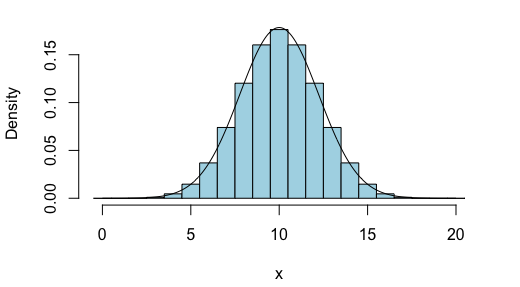
\includegraphics[scale=1]{BinomDist}
  \captionof{figure}{In this case, \(X=10\) is the mode.} 
\end{center}
\begin{example}{2018 TPJC JC2 H2 MYE P2 8}{}
  On average, 3.5\% of a certain brand of chocolate turn out misshapen. The chocolates are sold in packets of 25.
  \begin{enumerate}[label=(\roman*)]
    \item State, in context, two assumptions needed for the number of misshapen chocolates in a packet to be well modelled by a binomial distribution.
    \item Explain why one of the assumptions stated in part (i) may not hold in this context.
  \end{enumerate}
  \textit{Answer:}
  \begin{enumerate}[label=(\roman*)]
    \item 
    \begin{enumerate}[label=\arabic*.]
      \item Each chocolate is \emph{equally likely} (3.) to be misshapen.
      \item The event that a chocolate is misshapen is \emph{independent} (2.) of the event that another chocolate is misshapen.
    \end{enumerate}
    \item While on average, the probability that a chocolate is misshapen is 3.5\%, it is possible that there are more misshapen chocolates at certain times, possible due to equipment malfunction, which would mean the probability is not constant.\\[3mm]
    OR\\[3mm]
    Misshapen chocolates could be the result of equipment used and as the equipment used would not be the same for the same portion of the chocolate produced, whether a chocolate is misshapen may not be independent of another chocolate being misshapen.
  \end{enumerate}
\end{example}

\subfile{Subfiles/FMBsubfile.tex}

\chapter{Bibliography}
\begin{enumerate}
  \item Fig 6.1 Trapezium rule: \url{https://tex.stackexchange.com/a/110618}
  \item Fig 6.2 Simpson's rule: \url{https://tex.stackexchange.com/a/439119}
  \item Oscillatory behavior of DEs modelling physical phenomena Fig 15.2 \url{https://tikz.net/dynamics_oscillator/}
  \item Mode of a binomial distribution Fig 17.1 \url{https://math.oxford.emory.edu/site/math117/normalApproxToBinomial/}
\end{enumerate}

\end{document}